% Generated by Sphinx.
\def\sphinxdocclass{report}
\documentclass[a4paper,10pt,twoside]{sphinxmanual}
\usepackage[utf8]{inputenc}
\DeclareUnicodeCharacter{00A0}{\nobreakspace}
\usepackage{cmap}
\usepackage[T1]{fontenc}
\usepackage[french]{babel}
\usepackage{times}
\usepackage[Sonny]{fncychap}
\usepackage{longtable}
\usepackage{sphinx}
\usepackage{multirow}
\makeatletter 
  \fancypagestyle{normal}{ 
    \fancyhf{} 
    \fancyfoot[LE,RO]{{\py@HeaderFamily\thepage}} 
    \fancyfoot[LO]{{\py@HeaderFamily\nouppercase{\rightmark}}} 
    \fancyfoot[RE]{{\py@HeaderFamily\nouppercase{\leftmark}}} 
    \fancyhead[LE,RO]{{\py@HeaderFamily \@title}} % here's the change 
    \renewcommand{\headrulewidth}{0.4pt} 
    \renewcommand{\footrulewidth}{0.4pt} 
  } 
\makeatother


\title{Développement d'une application de gestion de cours avec AngularJS}
\date{30 mars 2015}
\release{}
\author{Keran Kocher}
\newcommand{\sphinxlogo}{}
\renewcommand{\releasename}{}
\makeindex

\makeatletter
\def\PYG@reset{\let\PYG@it=\relax \let\PYG@bf=\relax%
    \let\PYG@ul=\relax \let\PYG@tc=\relax%
    \let\PYG@bc=\relax \let\PYG@ff=\relax}
\def\PYG@tok#1{\csname PYG@tok@#1\endcsname}
\def\PYG@toks#1+{\ifx\relax#1\empty\else%
    \PYG@tok{#1}\expandafter\PYG@toks\fi}
\def\PYG@do#1{\PYG@bc{\PYG@tc{\PYG@ul{%
    \PYG@it{\PYG@bf{\PYG@ff{#1}}}}}}}
\def\PYG#1#2{\PYG@reset\PYG@toks#1+\relax+\PYG@do{#2}}

\expandafter\def\csname PYG@tok@ne\endcsname{\def\PYG@tc##1{\textcolor[rgb]{0.00,0.44,0.13}{##1}}}
\expandafter\def\csname PYG@tok@s\endcsname{\def\PYG@tc##1{\textcolor[rgb]{0.25,0.44,0.63}{##1}}}
\expandafter\def\csname PYG@tok@gi\endcsname{\def\PYG@tc##1{\textcolor[rgb]{0.00,0.63,0.00}{##1}}}
\expandafter\def\csname PYG@tok@gu\endcsname{\let\PYG@bf=\textbf\def\PYG@tc##1{\textcolor[rgb]{0.50,0.00,0.50}{##1}}}
\expandafter\def\csname PYG@tok@vc\endcsname{\def\PYG@tc##1{\textcolor[rgb]{0.73,0.38,0.84}{##1}}}
\expandafter\def\csname PYG@tok@s1\endcsname{\def\PYG@tc##1{\textcolor[rgb]{0.25,0.44,0.63}{##1}}}
\expandafter\def\csname PYG@tok@il\endcsname{\def\PYG@tc##1{\textcolor[rgb]{0.13,0.50,0.31}{##1}}}
\expandafter\def\csname PYG@tok@kt\endcsname{\def\PYG@tc##1{\textcolor[rgb]{0.56,0.13,0.00}{##1}}}
\expandafter\def\csname PYG@tok@c\endcsname{\let\PYG@it=\textit\def\PYG@tc##1{\textcolor[rgb]{0.25,0.50,0.56}{##1}}}
\expandafter\def\csname PYG@tok@se\endcsname{\let\PYG@bf=\textbf\def\PYG@tc##1{\textcolor[rgb]{0.25,0.44,0.63}{##1}}}
\expandafter\def\csname PYG@tok@ni\endcsname{\let\PYG@bf=\textbf\def\PYG@tc##1{\textcolor[rgb]{0.84,0.33,0.22}{##1}}}
\expandafter\def\csname PYG@tok@ss\endcsname{\def\PYG@tc##1{\textcolor[rgb]{0.32,0.47,0.09}{##1}}}
\expandafter\def\csname PYG@tok@nv\endcsname{\def\PYG@tc##1{\textcolor[rgb]{0.73,0.38,0.84}{##1}}}
\expandafter\def\csname PYG@tok@si\endcsname{\let\PYG@it=\textit\def\PYG@tc##1{\textcolor[rgb]{0.44,0.63,0.82}{##1}}}
\expandafter\def\csname PYG@tok@w\endcsname{\def\PYG@tc##1{\textcolor[rgb]{0.73,0.73,0.73}{##1}}}
\expandafter\def\csname PYG@tok@mo\endcsname{\def\PYG@tc##1{\textcolor[rgb]{0.13,0.50,0.31}{##1}}}
\expandafter\def\csname PYG@tok@nb\endcsname{\def\PYG@tc##1{\textcolor[rgb]{0.00,0.44,0.13}{##1}}}
\expandafter\def\csname PYG@tok@bp\endcsname{\def\PYG@tc##1{\textcolor[rgb]{0.00,0.44,0.13}{##1}}}
\expandafter\def\csname PYG@tok@ge\endcsname{\let\PYG@it=\textit}
\expandafter\def\csname PYG@tok@vg\endcsname{\def\PYG@tc##1{\textcolor[rgb]{0.73,0.38,0.84}{##1}}}
\expandafter\def\csname PYG@tok@nf\endcsname{\def\PYG@tc##1{\textcolor[rgb]{0.02,0.16,0.49}{##1}}}
\expandafter\def\csname PYG@tok@kp\endcsname{\def\PYG@tc##1{\textcolor[rgb]{0.00,0.44,0.13}{##1}}}
\expandafter\def\csname PYG@tok@kn\endcsname{\let\PYG@bf=\textbf\def\PYG@tc##1{\textcolor[rgb]{0.00,0.44,0.13}{##1}}}
\expandafter\def\csname PYG@tok@nc\endcsname{\let\PYG@bf=\textbf\def\PYG@tc##1{\textcolor[rgb]{0.05,0.52,0.71}{##1}}}
\expandafter\def\csname PYG@tok@mh\endcsname{\def\PYG@tc##1{\textcolor[rgb]{0.13,0.50,0.31}{##1}}}
\expandafter\def\csname PYG@tok@gp\endcsname{\let\PYG@bf=\textbf\def\PYG@tc##1{\textcolor[rgb]{0.78,0.36,0.04}{##1}}}
\expandafter\def\csname PYG@tok@kd\endcsname{\let\PYG@bf=\textbf\def\PYG@tc##1{\textcolor[rgb]{0.00,0.44,0.13}{##1}}}
\expandafter\def\csname PYG@tok@nn\endcsname{\let\PYG@bf=\textbf\def\PYG@tc##1{\textcolor[rgb]{0.05,0.52,0.71}{##1}}}
\expandafter\def\csname PYG@tok@sd\endcsname{\let\PYG@it=\textit\def\PYG@tc##1{\textcolor[rgb]{0.25,0.44,0.63}{##1}}}
\expandafter\def\csname PYG@tok@vi\endcsname{\def\PYG@tc##1{\textcolor[rgb]{0.73,0.38,0.84}{##1}}}
\expandafter\def\csname PYG@tok@no\endcsname{\def\PYG@tc##1{\textcolor[rgb]{0.38,0.68,0.84}{##1}}}
\expandafter\def\csname PYG@tok@o\endcsname{\def\PYG@tc##1{\textcolor[rgb]{0.40,0.40,0.40}{##1}}}
\expandafter\def\csname PYG@tok@cs\endcsname{\def\PYG@tc##1{\textcolor[rgb]{0.25,0.50,0.56}{##1}}\def\PYG@bc##1{\setlength{\fboxsep}{0pt}\colorbox[rgb]{1.00,0.94,0.94}{\strut ##1}}}
\expandafter\def\csname PYG@tok@cm\endcsname{\let\PYG@it=\textit\def\PYG@tc##1{\textcolor[rgb]{0.25,0.50,0.56}{##1}}}
\expandafter\def\csname PYG@tok@sh\endcsname{\def\PYG@tc##1{\textcolor[rgb]{0.25,0.44,0.63}{##1}}}
\expandafter\def\csname PYG@tok@gd\endcsname{\def\PYG@tc##1{\textcolor[rgb]{0.63,0.00,0.00}{##1}}}
\expandafter\def\csname PYG@tok@sx\endcsname{\def\PYG@tc##1{\textcolor[rgb]{0.78,0.36,0.04}{##1}}}
\expandafter\def\csname PYG@tok@nd\endcsname{\let\PYG@bf=\textbf\def\PYG@tc##1{\textcolor[rgb]{0.33,0.33,0.33}{##1}}}
\expandafter\def\csname PYG@tok@k\endcsname{\let\PYG@bf=\textbf\def\PYG@tc##1{\textcolor[rgb]{0.00,0.44,0.13}{##1}}}
\expandafter\def\csname PYG@tok@nt\endcsname{\let\PYG@bf=\textbf\def\PYG@tc##1{\textcolor[rgb]{0.02,0.16,0.45}{##1}}}
\expandafter\def\csname PYG@tok@gs\endcsname{\let\PYG@bf=\textbf}
\expandafter\def\csname PYG@tok@c1\endcsname{\let\PYG@it=\textit\def\PYG@tc##1{\textcolor[rgb]{0.25,0.50,0.56}{##1}}}
\expandafter\def\csname PYG@tok@ow\endcsname{\let\PYG@bf=\textbf\def\PYG@tc##1{\textcolor[rgb]{0.00,0.44,0.13}{##1}}}
\expandafter\def\csname PYG@tok@s2\endcsname{\def\PYG@tc##1{\textcolor[rgb]{0.25,0.44,0.63}{##1}}}
\expandafter\def\csname PYG@tok@kc\endcsname{\let\PYG@bf=\textbf\def\PYG@tc##1{\textcolor[rgb]{0.00,0.44,0.13}{##1}}}
\expandafter\def\csname PYG@tok@sc\endcsname{\def\PYG@tc##1{\textcolor[rgb]{0.25,0.44,0.63}{##1}}}
\expandafter\def\csname PYG@tok@mf\endcsname{\def\PYG@tc##1{\textcolor[rgb]{0.13,0.50,0.31}{##1}}}
\expandafter\def\csname PYG@tok@cp\endcsname{\def\PYG@tc##1{\textcolor[rgb]{0.00,0.44,0.13}{##1}}}
\expandafter\def\csname PYG@tok@gr\endcsname{\def\PYG@tc##1{\textcolor[rgb]{1.00,0.00,0.00}{##1}}}
\expandafter\def\csname PYG@tok@m\endcsname{\def\PYG@tc##1{\textcolor[rgb]{0.13,0.50,0.31}{##1}}}
\expandafter\def\csname PYG@tok@sr\endcsname{\def\PYG@tc##1{\textcolor[rgb]{0.14,0.33,0.53}{##1}}}
\expandafter\def\csname PYG@tok@kr\endcsname{\let\PYG@bf=\textbf\def\PYG@tc##1{\textcolor[rgb]{0.00,0.44,0.13}{##1}}}
\expandafter\def\csname PYG@tok@sb\endcsname{\def\PYG@tc##1{\textcolor[rgb]{0.25,0.44,0.63}{##1}}}
\expandafter\def\csname PYG@tok@mi\endcsname{\def\PYG@tc##1{\textcolor[rgb]{0.13,0.50,0.31}{##1}}}
\expandafter\def\csname PYG@tok@na\endcsname{\def\PYG@tc##1{\textcolor[rgb]{0.25,0.44,0.63}{##1}}}
\expandafter\def\csname PYG@tok@go\endcsname{\def\PYG@tc##1{\textcolor[rgb]{0.20,0.20,0.20}{##1}}}
\expandafter\def\csname PYG@tok@err\endcsname{\def\PYG@bc##1{\setlength{\fboxsep}{0pt}\fcolorbox[rgb]{1.00,0.00,0.00}{1,1,1}{\strut ##1}}}
\expandafter\def\csname PYG@tok@nl\endcsname{\let\PYG@bf=\textbf\def\PYG@tc##1{\textcolor[rgb]{0.00,0.13,0.44}{##1}}}
\expandafter\def\csname PYG@tok@gt\endcsname{\def\PYG@tc##1{\textcolor[rgb]{0.00,0.27,0.87}{##1}}}
\expandafter\def\csname PYG@tok@mb\endcsname{\def\PYG@tc##1{\textcolor[rgb]{0.13,0.50,0.31}{##1}}}
\expandafter\def\csname PYG@tok@gh\endcsname{\let\PYG@bf=\textbf\def\PYG@tc##1{\textcolor[rgb]{0.00,0.00,0.50}{##1}}}

\def\PYGZbs{\char`\\}
\def\PYGZus{\char`\_}
\def\PYGZob{\char`\{}
\def\PYGZcb{\char`\}}
\def\PYGZca{\char`\^}
\def\PYGZam{\char`\&}
\def\PYGZlt{\char`\<}
\def\PYGZgt{\char`\>}
\def\PYGZsh{\char`\#}
\def\PYGZpc{\char`\%}
\def\PYGZdl{\char`\$}
\def\PYGZhy{\char`\-}
\def\PYGZsq{\char`\'}
\def\PYGZdq{\char`\"}
\def\PYGZti{\char`\~}
% for compatibility with earlier versions
\def\PYGZat{@}
\def\PYGZlb{[}
\def\PYGZrb{]}
\makeatother

\renewcommand\PYGZsq{\textquotesingle}

\begin{document}

\maketitle
\tableofcontents
\phantomsection\label{index::doc}



\chapter{Introduction}
\label{introduction:developpement-d-une-application-de-gestions-de-cours-avec-angularjs}\label{introduction::doc}\label{introduction:introduction}\setcounter{page}{3}
Les chapitres qui suivent décrivent le développement d'une application web complète et fonctionnelle. Mon choix s'est porté sur ce travail pour plusieurs raisons. Tout d'abord, l'informatique est une de mes plus grandes passions et ce projet est l'occasion de m'épanouir dans ce domaine. En effet, j'ai l'opportunité d'acquérir des connaissances supplémentaires et de progresser dans la programmation web en profitant de l'expertise d'un professeur. Ensuite, le cadre de groupe offre la possibilité d'apprendre à travailler à plusieurs pour atteindre un objectif commun, en l'occurence le développement d'une plateforme d'e-learning. L'application décrite dans ce document est un outil de gestion et de visionnage de cours. Elle propose aux enseignants de rédiger du contenu théorique, qui peut ensuite être visionné par des élèves. Ainsi, dans le cadre de ses classes, un professeur peut écrire un cours, en complément de son support habituel, afin d'appronfondir une matière ou d'aider des élèves en difficulté. Il a entre les mains un outil puissant. En effet, outre la possibilité d'aider ses propres étudiants, l'enseignant a également une plateforme pour exposer ses connaissances et les partager à un public plus large que l'école. De plus, il a tout intérêt à encourager ses élèves à s'inscrire sur le site. Effectivement, d'une part le site permet aux utilisateurs d'ajouter des cours à leurs favoris afin de les retrouver sans effort; d'autre part, sur chaque cours est offerte la possibilité de marquer une page comme lue ou à relire. Par conséquent, chaque élève sait où il se situe dans son apprentissage de la matière et peut facilement progresser.

Pour atteindre l'objectif de l'application, on utilise une technologie en particulier. Il s'agit d'AngularJS, un outil développé par Google. Le projet s'articule principalement autour de cette technologie qui permet de construire des sites web rapides et agréables à utiliser. Le documentation qui suit sert à expliquer les bases d'AngularJS et son intégration avec Django, ainsi que d'autres technologies annexes. Ainsi, au terme de ce travail écrit, le lecteur est capable de comprendre le code source de l'application afin de pouvoir le réutiliser, le maintenir ou l'étendre.


\chapter{Démarrage}
\label{start::doc}\label{start:demarrage}
\textbf{Prérequis}
\begin{itemize}
\item {} 
Python 3 et pip installés

\end{itemize}

\textbf{Installer Django et les dépendances}

\code{pip3 install -r requirements.txt}

De plus, il faut encore installer ces paquets sur la machine:
\begin{itemize}
\item {} 
pandoc

\item {} 
pdflatex

\end{itemize}

\textbf{Lancer les migrations}

\code{python3 manage.py migrate}

\textbf{Créer un super utilisateur}

S'il y a besoin de se connecter à la zone d'administration (\code{/admin})

\code{python3 manage.py createsuperuser}

\textbf{Lancer le serveur Django}

\code{python3 manage.py runserver}

\textbf{Données}
\begin{itemize}
\item {} 
Créer les données nécessaires: \code{python3 manage.py seed}

\item {} 
Finalement, vous pouvez vous rendre sur l'URL \code{/courses} et profiter des fonctionnalités.

\item {} 
Identifiant pour se connecter en tant qu'enseignant: \code{smith.john} et \code{12341}

\item {} 
Identifiant pour se connecter en tant qu'étudiant: \code{dupont.alfred} et \code{12341}

\end{itemize}

\textbf{Tests}

Pour lancer les tests, installer d'abord Protractor (ne pas lancer le serveur webdriver): \href{http://angular.github.io/protractor/\#/tutorial}{http://angular.github.io/protractor/\#/tutorial}

Ensuite, lancer la commande \code{python3 manage.py tests}.


\chapter{AngularJS}
\label{angularjs::doc}\label{angularjs:angularjs}

\section{Introduction}
\label{angularjs:introduction}
AngularJS est un framework JavaScript créé et maintenu depuis 2009 par Google, l'entreprise à l'origine du populaire moteur de recherche, du client Gmail mais aussi de beaucoup d'outils pour les développeurs. Outre le fait de créer des outils de programmation comme AngularJS, Google propose des outils d'analyse (\href{http://google.com/analytics}{Google Analytics} \footnote{
\href{http://google.com/analytics}{http://google.com/analytics}. Consulté le 25 décembre 14.
}), de stockage (\href{https://cloud.google.com}{Google Cloud} \footnote{
\href{https://cloud.google.com}{https://cloud.google.com}. Consulté le 25 décembre 14.
}), ou encore des serveurs pour héberger des applications. Une entreprise très présente non seulement dans le domaine public, mais également dans le soutien et la recherche des technologies informatiques. Pour revenir au sujet qui nous intéresse, l'équipe de Google a donc développé le framework AngularJS. Un framework est un ensemble de structures et d'outils programmés dans un langage et réutilisables, qui permettent de faciliter la construction d'applications. On trouve par exemple chez PHP le framework \href{http://symfony.com}{Symfony} \footnote{
\href{http://symfony.com}{http://symfony.com}. Consulté le 25 décembre 14.
}, chez Ruby \href{http://rubyonrails.com}{Ruby on Rails} \footnote{
\href{http://rubyonrails.com}{http://rubyonrails.com}. Consulté le 25 décembre 14.
}, chez Python \emph{Django} que nous utilisons pour notre site web. Finalement, chez JavaScript on trouve \emph{AngularJS}, mais encore comme concurrents \href{http://emberjs.com}{Ember} \footnote{
\href{http://emberjs.com}{http://emberjs.com}. Consulté le 25 décembre 14.
} ou \href{http://facebook.github.io/react/}{React} \footnote{
\href{http://facebook.github.io/react}{http://facebook.github.io/react}. Consulté le 10 mars 15.
}.

AngularJS permet de développer une application web complète. C'est-à-dire qu'il offre plusieurs outils indispensables. Tout d'abord, un système de routes qui permet de lier des URL avec des pages différentes. En clair, l'on peut ordonner à notre application que lorsque l'utilisateur entre \code{monsite.com/contact} dans son navigateur, le fichier \code{contact.html} doit être affiché. Il y a aussi la prise en charge des formulaires, avec la possibilité de récupérer les informations entrées par l'utilisateur ou de faire une validation du formulaire, c'est-à-dire de vérifier les informations entrées. En revanche, AngularJS ne sait pas comment communiquer directement avec une base de données - une base de données est l'endroit où sont stockées les données persistantes -, il est seulement capable d'utiliser les données d'une base de données fournie par un serveur intermédiaire. Les bases de données sont souvent indispensables, car elles permettent de concevoir des sites web dynamiques. Il est donc nécessaire d'utiliser un autre langage avec AngularJS. Django jouera ce rôle mais nous éclaircirons ce concept plus tard lorsque nous étudierons son intégration avec Angular.

Pour bien comprendre la documentation du projet, il faut savoir ce qu'est Django. Comme mentionné précédemment, il s'agit d'un framework Python. Il est spécialisé dans la création de site web et est le leader face à ses concurrents comme \href{http://www.turbogears.org/}{Turbo Gears} \footnote{
\href{http://www.turbogears.org}{http://www.turbogears.org}. Consulté le 25 décembre 14.
}. Django est ce que nous utilisons principalement pour créer notre application web. Créer un site web avec Python seulement est difficile et peu pratique, un framework est  quasiment indispensable. Effectivement, Django fournit les outils nécessaires pour créer des pages HTML, communiquer avec une base de données, gérer les URLs, etc. Pour comprendre les exemples Django qui apparaitront, il faut savoir que celui-ci utilise le modèle MVC - modèle, vue, contrôleur - qui est expliqué dans la section suivante. La particularité est que Django a changé les termes: \emph{modèle} reste \emph{modèle}, \emph{vue} est égale à \emph{template} et \emph{contrôleur} est égal à \emph{vue}.

\begin{tabulary}{\linewidth}{|L|L|}
\hline
\textsf{\relax 
MVC
} & \textsf{\relax 
MVT (Django)
}\\
\hline
Modèle
 & 
Modèle
\\

Vue
 & 
Template
\\

Contrôleur
 & 
Vue
\\
\hline\end{tabulary}



\section{Spécificités et avantages}
\label{angularjs:specificites-et-avantages}
Qu'est-ce qui démarque AngularJS de ses concurrents ? En bref, quelles sont ses fonctionnalités, qui facilitent tant la vie des développeurs ? La première chose à connaitre d'AngularJS est qu'il encourage le modèle MVC - modèle, vue, contrôleur. Il s'agit en fait de séparer dans notre application ces trois composants. Grossièrement, le modèle est la partie qui gère les données de l'application, la vue s'occupe de ce qui est affiché à l'utilisateur et le contrôleur est la partie qui relie le modèle à la vue. Il va chercher les données dans les modèles pour les donner à la vue qui les affiche et, vice-versa, il reçoit les données de la vue, par un formulaire par exemple, pour mettre à jour le modèle. Un principe très important dans ce motif de programmation est que le minimum de code logique doit se trouver dans les vues. Elles doivent se contenter d'afficher, car toutes les opérations se font idéalement dans les contrôleurs ou les modèles. L'avantage de cette organisation est une compréhension plus aisée et une modularité du code.

Dans la suite de cette section nous allons nous intéresser à quelques fonctionnalités clés d'AngularJS.


\subsection{Du HTML expressif}
\label{angularjs:du-html-expressif}
Abordons d'abord les vues. Le premier ``miracle'' du framework est de transformer le HTML statique en un langage expressif et dynamique. A la base, le HTML est une syntaxe qui permet de structurer une page web à l'aide de balises qui définissent leur contenu, comme par exemple les balises qui délimitent les paragraphes, les titres, les images, etc. Traditionnellement, on utilise un autre langage, comme Python, pour transformer la page et y insérer le contenu dynamique qui provient de la base de données. Concrètement, il pourrait s'agir d'afficher une liste d'articles dans une page. Si l'on travaille avec Django, on assigne à une variable \code{articles} tous les articles à l'aide d'une requête SQL; SQL est le langage pour communiquer avec une base de données relationnelle. On fait ensuite une boucle dans la page HTML et l'on affiche le titre ainsi que le contenu de chaque article.

\begin{Verbatim}[commandchars=\\\{\}]
\PYG{n+nt}{\PYGZlt{}html}\PYG{n+nt}{\PYGZgt{}}
    \PYG{n+nt}{\PYGZlt{}head}\PYG{n+nt}{\PYGZgt{}}\PYG{n+nt}{\PYGZlt{}/head\PYGZgt{}}
    \PYG{n+nt}{\PYGZlt{}body}\PYG{n+nt}{\PYGZgt{}}
        \PYG{n+nt}{\PYGZlt{}div} \PYG{n+na}{id=}\PYG{l+s}{\PYGZdq{}articles\PYGZdq{}}\PYG{n+nt}{\PYGZgt{}}
            \PYGZob{}\PYGZpc{} for article in articles \PYGZpc{}\PYGZcb{}
                \PYG{n+nt}{\PYGZlt{}h1}\PYG{n+nt}{\PYGZgt{}}\PYGZob{}\PYGZob{} article.titre \PYGZcb{}\PYGZcb{}\PYG{n+nt}{\PYGZlt{}/h1\PYGZgt{}}
                \PYG{n+nt}{\PYGZlt{}p}\PYG{n+nt}{\PYGZgt{}}\PYGZob{}\PYGZob{} article.contenu \PYGZcb{}\PYGZcb{}\PYG{n+nt}{\PYGZlt{}/p\PYGZgt{}}
            \PYGZob{}\PYGZpc{} endfor \PYGZpc{}\PYGZcb{}
        \PYG{n+nt}{\PYGZlt{}/div\PYGZgt{}}
    \PYG{n+nt}{\PYGZlt{}body}\PYG{n+nt}{\PYGZgt{}}
\PYG{n+nt}{\PYGZlt{}html}\PYG{n+nt}{\PYGZgt{}}
\end{Verbatim}

Les balises \code{\{\% \%\}} et \code{\{\{ \}\}} signifient simplement que ce n'est plus du HTML, mais que du code Django est à l'intérieur et doit être exécuté par le serveur.

Avec AngularJS, le modèle est légèrement différent. En effet, on trouve dans le framework ce que l'on appelle des directives, un concept spécifique à Angular. Ce sont des balises ou des attributs HTML supplémentaires que fournit AngularJS. On peut les ajouter à notre page et elles effectuent différentes actions selon leur rôle. Pour reprendre l'exemple des articles, pour faire une boucle, on utilise la directive \code{ng-repeat}. On l'utilise comme un simple attribut HTML.

\begin{Verbatim}[commandchars=\\\{\}]
\PYG{n+nt}{\PYGZlt{}html}\PYG{n+nt}{\PYGZgt{}}
    \PYG{n+nt}{\PYGZlt{}head}\PYG{n+nt}{\PYGZgt{}}\PYG{n+nt}{\PYGZlt{}/head\PYGZgt{}}
    \PYG{n+nt}{\PYGZlt{}body}\PYG{n+nt}{\PYGZgt{}}
        \PYG{n+nt}{\PYGZlt{}div} \PYG{n+na}{id=}\PYG{l+s}{\PYGZdq{}articles\PYGZdq{}} \PYG{n+na}{ng\PYGZhy{}repeat=}\PYG{l+s}{\PYGZdq{}article in articles\PYGZdq{}}\PYG{n+nt}{\PYGZgt{}}
            \PYG{n+nt}{\PYGZlt{}h1}\PYG{n+nt}{\PYGZgt{}}\PYGZob{}\PYGZob{} article.titre \PYGZcb{}\PYGZcb{}\PYG{n+nt}{\PYGZlt{}/h1\PYGZgt{}}
            \PYG{n+nt}{\PYGZlt{}p}\PYG{n+nt}{\PYGZgt{}}\PYGZob{}\PYGZob{} article.contenu \PYGZcb{}\PYGZcb{}\PYG{n+nt}{\PYGZlt{}/p\PYGZgt{}}
        \PYG{n+nt}{\PYGZlt{}/div\PYGZgt{}}
    \PYG{n+nt}{\PYGZlt{}body}\PYG{n+nt}{\PYGZgt{}}
\PYG{n+nt}{\PYGZlt{}html}\PYG{n+nt}{\PYGZgt{}}
\end{Verbatim}

A l'instar de Django, les doubles accolades signifient que l'on veut exécuter du code Angular/JavaScript à l'intérieur. Ici on affiche simplement une variable, mais l'on pourrait également faire un calcul et afficher le résultat: \code{\{\{ 1 + 2 \}\}}. En revanche, AngularJS est exécuté côté client, contrairement à Django qui est côté serveur.

Comme précédemment, l'on a assigné une variable avec tous les articles. Cependant cette fois, la boucle se fait directement en utilisant la directive \code{ng-repeat} qui se confond avec la syntaxe HTML. A l'intérieur de l'attribut, il faut utiliser la syntaxe Angular pour faire la boucle: \code{article in articles}. On lui demande de parcourir la variable \code{articles} et d'utiliser comme variable temporaire \code{article} pour chaque article parcouru. Il existe beaucoup d'autre directives dans AngularJS, par exemple pour réagir au clic d'une souris sur un élément, pour afficher ou cacher des sections. Il est aussi possible de créer ses directives personnalisées avec le comportement désiré. Créer ses propres directives permet, soit d'avoir un code plus clair, soit d'éviter la répétition. Dans les deux cas, cette fonctionnalité est très utile et puissante.

A cause de ces directives, l'on parle d'HTML expressif. En effet, avec celles-ci, le HTML ne décrit pas seulement le contenu, mais aussi le comportement de l'application web et sa manière de fonctionner. L'on sait ainsi clairement et rapidement en regardant notre page HTML les fonctionnalités que l'on a implémentées sur celle-ci, ce qui rend plus facile la vue d'ensemble de son application.


\subsection{Two-way data binding}
\label{angularjs:two-way-data-binding}
La deuxième fonctionnalité majeure d'AngularJS est ce que l'on appelle \emph{two-way data binding} ou en français \emph{la liaison des données à double sens}. Derrière cette mystérieuse expression se cache la manière qu'utilise le framework pour relier le modèle et la vue. Le système habituel est comme suit; l'on génère les vues en fonction de ce qui se trouve dans le modèle, comme dans l'exemple précédent où l'on cherche des articles dans la \emph{BD} pour ensuite générer une page. Lorsque le modèle change, un article est ajouté par exemple, la vue ne se met pas à jour. On doit la générer à nouveau pour voir le nouvel article. De plus, si l'utilisateur remplit un formulaire pour ajouter un nouvel article, le modèle ne change pas, tant que le formulaire n'a pas été traité. On appelle logiquement ce système \emph{one-way data binding}. Le schéma qui suit illustre ce principe. Pour générer une vue pour l'utilisateur, le gabarit et le modèle doivent être fusionnés et chaque fois qu'un changement est fait, l'on doit refaire le même processus.
\begin{figure}[htbp]
\centering
\capstart

\scalebox{0.600000}{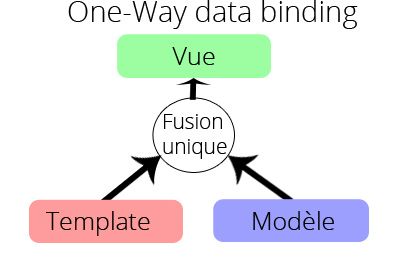
\includegraphics{One_Way_Data_Binding.jpg}}
\caption{One-way data binding}\end{figure}

Avec Angular, le principe est plus intelligent. Les vues se génèrent effectivement en fonction des modèles, en revanche, si le modèle change, la vue se met automatiquement à jour sans avoir effectué un nouveau rendu de la page. Si un utilisateur fait un changement dans la vue, le modèle change également. Les deux entités sont donc toujours synchronisées grâce à ce mécanisme du framework. La vue met à jour le modèle et le modèle met à jour la vue, continuellement.
\begin{figure}[htbp]
\centering
\capstart

\scalebox{0.600000}{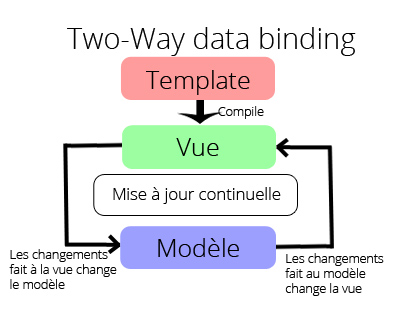
\includegraphics{Two_Way_Data_Binding.jpg}}
\caption{Two-way data binding}\end{figure}

Cette fonctionnalité facilite énormément la vie du développeur. Imaginons un système de commentaires. Il y a une liste de commentaires et un formulaire pour en rajouter. Pour le développeur, il suffit de relier le formulaire au modèle. Ensuite, au fur et à mesure que l'utilisateur tape son commentaire, le modèle est mis à jour et contient le nouveau commentaire. Il peut déjà s'afficher dans la liste. Voici un exemple de code qui permet de cacher ou d'afficher une portion de page à l'aide d'un bouton.

\begin{Verbatim}[commandchars=\\\{\}]
\PYG{c}{\PYGZlt{}!\PYGZhy{}\PYGZhy{}}\PYG{c}{ index.html }\PYG{c}{\PYGZhy{}\PYGZhy{}\PYGZgt{}}
\PYG{n+nt}{\PYGZlt{}html} \PYG{n+na}{ng\PYGZhy{}app=}\PYG{l+s}{\PYGZdq{}DemoApp\PYGZdq{}}\PYG{n+nt}{\PYGZgt{}}
    \PYG{n+nt}{\PYGZlt{}head}\PYG{n+nt}{\PYGZgt{}}\PYG{n+nt}{\PYGZlt{}/head\PYGZgt{}}
    \PYG{n+nt}{\PYGZlt{}body} \PYG{n+na}{ng\PYGZhy{}controller=}\PYG{l+s}{\PYGZdq{}IndexController\PYGZdq{}}\PYG{n+nt}{\PYGZgt{}}
        \PYG{c}{\PYGZlt{}!\PYGZhy{}\PYGZhy{}}\PYG{c}{ section affichée selon la variable \PYGZdq{}affiche\PYGZdq{} grâce à la directive ng}\PYG{c}{\PYGZhy{}}\PYG{c}{show }\PYG{c}{\PYGZhy{}\PYGZhy{}\PYGZgt{}}
        \PYG{n+nt}{\PYGZlt{}div} \PYG{n+na}{ng\PYGZhy{}show=}\PYG{l+s}{\PYGZdq{}affiche\PYGZdq{}}\PYG{n+nt}{\PYGZgt{}}
           \PYG{n+nt}{\PYGZlt{}h1}\PYG{n+nt}{\PYGZgt{}}Je suis une section cachée !\PYG{n+nt}{\PYGZlt{}/h1\PYGZgt{}}
           \PYG{n+nt}{\PYGZlt{}p}\PYG{n+nt}{\PYGZgt{}}Mais je ne cache rien d\PYGZsq{}intéressant...\PYG{n+nt}{\PYGZlt{}p}\PYG{n+nt}{\PYGZgt{}}
        \PYG{n+nt}{\PYGZlt{}/div\PYGZgt{}}
        \PYG{c}{\PYGZlt{}!\PYGZhy{}\PYGZhy{}}\PYG{c}{ bouton qui affiche/cache la section. Appelle la fonction toggle()}
\PYG{c}{        grâce à la directive ng}\PYG{c}{\PYGZhy{}}\PYG{c}{click }\PYG{c}{\PYGZhy{}\PYGZhy{}\PYGZgt{}}
        \PYG{n+nt}{\PYGZlt{}button} \PYG{n+na}{type=}\PYG{l+s}{\PYGZdq{}button\PYGZdq{}} \PYG{n+na}{ng\PYGZhy{}click=}\PYG{l+s}{\PYGZdq{}toggle()\PYGZdq{}}\PYG{n+nt}{\PYGZgt{}}Afficher/Cacher\PYG{n+nt}{\PYGZlt{}/button\PYGZgt{}}
    \PYG{n+nt}{\PYGZlt{}body}\PYG{n+nt}{\PYGZgt{}}
\PYG{n+nt}{\PYGZlt{}html}\PYG{n+nt}{\PYGZgt{}}
\end{Verbatim}

\begin{Verbatim}[commandchars=\\\{\}]
\PYG{c+c1}{// index\PYGZus{}controller.js}
\PYG{c+c1}{// On crée une application Angular}
\PYG{k+kd}{var} \PYG{n+nx}{app} \PYG{o}{=} \PYG{n+nx}{angular}\PYG{p}{.}\PYG{n+nx}{module}\PYG{p}{(}\PYG{l+s+s2}{\PYGZdq{}DemoApp\PYGZdq{}}\PYG{p}{)}\PYG{p}{;}

\PYG{c+c1}{// On crée un contrôleur Angular}
\PYG{n+nx}{app}\PYG{p}{.}\PYG{n+nx}{controller}\PYG{p}{(}\PYG{l+s+s2}{\PYGZdq{}IndexController\PYGZdq{}}\PYG{p}{,} \PYG{k+kd}{function}\PYG{p}{(}\PYG{n+nx}{\PYGZdl{}scope}\PYG{p}{)} \PYG{p}{\PYGZob{}}

    \PYG{c+c1}{// variable utilisée dans ng\PYGZhy{}show=\PYGZdq{}affiche\PYGZdq{}}
    \PYG{n+nx}{\PYGZdl{}scope}\PYG{p}{.}\PYG{n+nx}{affiche} \PYG{o}{=} \PYG{k+kc}{false}\PYG{p}{;}

    \PYG{c+c1}{// fonction appelée lorsque l\PYGZsq{}on clique sur le bouton}
    \PYG{n+nx}{\PYGZdl{}scope}\PYG{p}{.}\PYG{n+nx}{toggle} \PYG{o}{=} \PYG{k+kd}{function}\PYG{p}{(}\PYG{p}{)} \PYG{p}{\PYGZob{}}
        \PYG{n+nx}{\PYGZdl{}scope}\PYG{p}{.}\PYG{n+nx}{affiche} \PYG{o}{=} \PYG{o}{!}\PYG{n+nx}{\PYGZdl{}scope}\PYG{p}{.}\PYG{n+nx}{affiche}
    \PYG{p}{\PYGZcb{}}\PYG{p}{;}

\PYG{p}{\PYGZcb{}}\PYG{p}{)}\PYG{p}{;}
\end{Verbatim}

Tout d'abord, l'on affiche une section selon une variable booléenne \code{affiche} et l'on assigne à la variable la valeur \code{false} par défaut. La section est donc cachée. Puis l'on ajoute un bouton qui exécute une fonction qui change la valeur de notre variable \code{affiche} de \code{false} à \code{true} et vice-versa. La section s'affiche ou se cache selon son état lorsque l'on clique sur le bouton. Plusieurs directives sont utilisées dans l'exemple. \code{ng-app} signale à AngularJS qu'il faut analyser et compiler cette page. \code{ng-controller} signale qu'il faut utiliser le contrôleur \code{IndexController} qui est défini dans le fichier JavaScript et exécuter le code à l'intérieur. \code{ng-show} montre ou non la section selon la contenu de la variable booléenne \code{affiche} et \code{ng-click} exécute la fonction \code{toggle()} lorsque que l'on clique sur le bouton.


\subsection{Et plus encore...}
\label{angularjs:et-plus-encore}
Il y a évidemment encore d'autres avantages à utiliser ce framework, notamment les injections de dépendances et l'extensibilité d'AngularJS, mais nous avons vu les deux principales différences dans le monde des frameworks JavaScript.


\chapter{Fonctionnalités}
\label{functionalities::doc}\label{functionalities:fonctionnalites}

\section{Les professeurs}
\label{functionalities:les-professeurs}
Les comptes ``professeurs'' du site web ont la possibilité de rédiger des cours complets qui sont ensuite consultables par les autres utilisateurs du site, principalement des élèves. L'objectif est de pouvoir offrir du contenu théorique d'apprentissage en complément de partie pratique. Les enseignants disposent d'un outil formidable pour écrire des compléments au cours de base, afin d'approfondir des éléments ou de les clarifier pour les élèves en difficulté.


\subsection{Création}
\label{functionalities:creation}
La première étape du processeur de rédaction consiste à créer le cours en entrant les informations basiques du cours, à savoir le nom, la description, la catégorie et la difficulté. En ce qui concerne le nom et la description, ces champs parlent d'eux-mêmes. Il s'agit de saisir les informations pertinentes qui correspondent au contenu du cours afin que celui-ci puisse attirer les utilisateurs. Pour la catégorie, il faut choisir parmi les chapitres proposés, qui sont eux-mêmes regroupés par thèmes. Par exemple, un cours sur ``les tangentes'' se place dans le chapitre ``Les cercles'' qui lui-même est dans le thème ``Géométrie''. Ainsi, les différentes ressources du site sont classées, et l'élève retrouve facilement la matière qui l'intéresse. Finalement, le professeur choisit la difficulté, sur une échelle de 1 à 3, de facile à difficile.

Tous les champs sont obligatoires. Une fois les champs dûment complétés, il suffit à l'auteur de cliquer sur le bouton ``Envoyer'' (1) pour être redirigé sur la page de rédaction où il peut commencer à écrire.
\begin{figure}[htbp]
\centering
\capstart

\scalebox{0.500000}{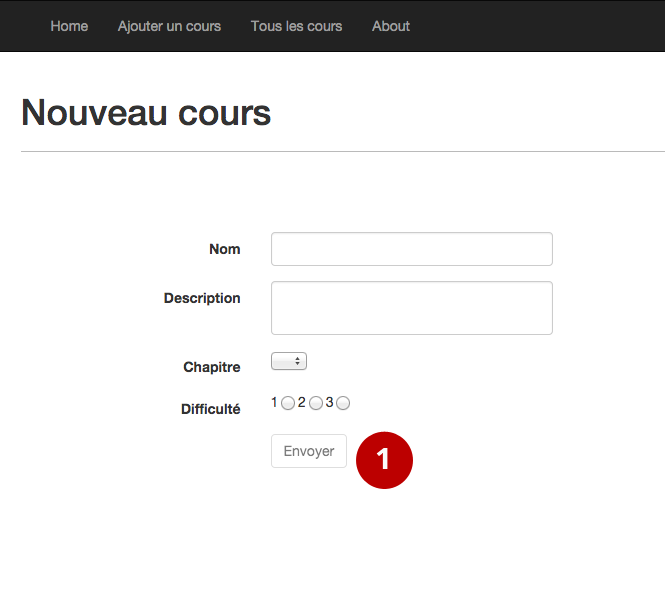
\includegraphics{new.png}}
\caption{Création d'un cours}\end{figure}


\subsection{Rédaction}
\label{functionalities:redaction}

\subsubsection{Structurer son cours}
\label{functionalities:structurer-son-cours}
Pour structurer son cours, l'auteur peut tout d'abord créer plusieurs pages ayant chacune un titre (1). Ensuite, dans chacune de ces pages, le contenu se découpe en plusieurs sections avec un titre (2) et un contenu (3). L'avantage de cette structure est que le site génère automatiquement un sommaire interactif du cours, en se basant sur le titre des pages et celui des sections.

L'action de créer des pages ou des sections et de modifier leur contenu se fait de manière claire, simple et surtout rapide. Le professeur travaille sans jamais devoir recharger sa page, action généralement lente. Pour ajouter une section, un bouton se trouve en bas de page (4). En cliquant dessus, une nouvelle zone d'édition va simplement apparaître. En bas de la page se trouvent le bouton (5) pour ajouter une nouvelle page, ainsi que la liste des différentes pages déjà créées (6). L'on peut donc, soit créer une page en cliquant sur le bouton (5), ce qui a pour effet d'afficher une nouvelle page vierge, soit encore naviguer entre les pages du cours pour éditer leur contenu en cliquant sur le numéro des pages (6). Il se peut aussi que l'on veuille réorganiser les sections dans un ordre différent, ou supprimer une section. Cette action est tout à fait possible; à côté de chacune des sections se trouve trois boutons (7): celui pour supprimer la section et les deux autres pour la monter ou la descendre. Lorsque l'on clique sur l'un des trois, la page est mise à jour automatiquement et instantanément.

En ce qui concerne l'enregistrement, il se fait automatiquement toutes les 30 secondes. De plus, au cas où l'on crée ou change une page, ou réorganise les sections, lorsque l'on prévisualise le cours, publie ou retire, de même que si l'on quitte la page, le cours est aussi sauvegardé. Il y a un bouton ``Enregistrer'' (8) en haut de la page pour faire une sauvegarde manuelle. L'heure du dernier enregistrement est affichée à la gauche du bouton.


\subsubsection{Mise en forme}
\label{functionalities:mise-en-forme}
Pour mettre en forme le texte de son cours, le rédacteur utilise la syntaxe populaire \emph{Markdown}. La syntaxe consiste à mettre dans le texte des marques avec des symboles qui sont ensuite interprétés, soit comme des titres, des images, du texte gras, etc. Par exemple, pour mettre en italique, on entoure un mot avec ``*''. Ainsi l'on peut facilement souligner du texte, ajouter des images, faire des tableaux et des listes, etc. S'il n'est pas encore à l'aise avec la syntaxe, le professeur peut à tout moment cliquer sur le bouton d'aide (9) en haut de la page, représenté par un point d'interrogation. Il découvre alors des liens pour avoir un rapide aperçu de l'ensemble des fonctionnalités du \emph{Markdown}.

De plus, comme les cours visent avant tout un contenu mathématique, l'auteur peut (et doit) baliser le contenu mathématique. Ainsi celui-ci est formaté pour le rendu final et donc correctement affiché. La notation à utiliser pour les formules mathématique est celle du populaire format \emph{LaTex}. Par conséquent, il suffit au professeur de mettre les balises et d'écrire ensuite sa formule mathématique en utilisant la syntaxe \emph{LaTex} (10). Il y a deux types de balises. \code{\textbackslash{}(} ... \code{\textbackslash{})} est utilisée pour intégrer des mathématiques directement dans le texte. La balise \code{\textbar{}\textbar{}} est utilisée pour un affichage en bloc, c'est-à-dire que la formule est sur une nouvelle ligne, séparée du texte. A l'instar du \emph{Markdown}, on peut se référer à la section d'aide pour se familiariser avec la syntaxe \emph{LaTex} (9).

L'auteur n'ayant pas un aperçu direct du rendu de son texte, il peut cliquer sur le bouton en haut ``Aperçu'' (11) pour regarder comment le contenu est réellement affiché. Il n'a pas besoin de sauvegarder avant de faire l'aperçu. Une fois sur la page de prévisualisation, il peut retourner à la rédaction du cours en cliquant sur ``Retour'' en haut à gauche.


\subsubsection{Ajouter des médias}
\label{functionalities:ajouter-des-medias}
Evidemment, l'auteur peut inclure des vidéos et des images pour enrichir son contenu. Il peut ajouter une image provenant d'internet en utilisant la syntaxe \emph{Markdown} et le lien de l'image, tandis que pour la vidéo il peut en inclure une provenant de Youtube avec le même procédé que pour l'image (voir aide \emph{Markdown}).


\subsubsection{Modifier les informations de base}
\label{functionalities:modifier-les-informations-de-base}
Lorsque l'enseignant désire modifier les informations saisies lors du processus de création, il peut cliquer sur le lien ``Editer'' (12) à côté du titre du cours. Il est alors sur une page avec le même formulaire qu'à la création du cours. L'auteur peut donc éditer le titre, la description, la catégorie et la difficulté et cliquer sur ``Envoyer''. Finalement, il est possible de retourner sur la page de rédaction en cliquant sur ``Retour'' en haut à gauche.


\subsubsection{Publier un cours}
\label{functionalities:publier-un-cours}
Par défaut, le cours créé par un professeur n'est pas visible par les utilisateurs du site, afin de laisser à l'auteur le temps de rédiger le cours en entier. Lorsqu'il estime le cours prêt, il peut tout simplement cliquer sur le bouton ``Publier'' (13) tout en haut de la page pour rendre le cours visible. Il peut bien sûr retirer son cours de la liste à tout moment s'il désire apporter des modifications ou estime qu'il ne doit plus être lisible sur le site.
\begin{figure}[htbp]
\centering
\capstart

\scalebox{0.600000}{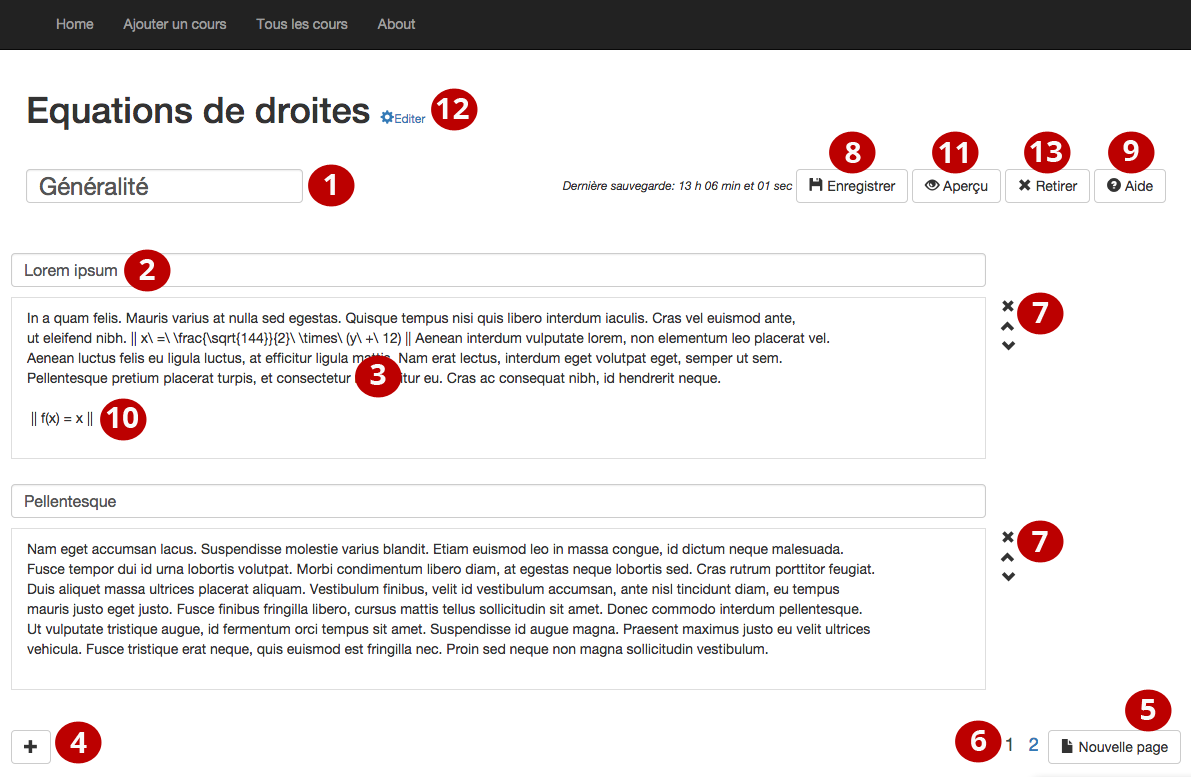
\includegraphics{edit.png}}
\caption{Edition d'un cours}\end{figure}


\subsubsection{Retrouver son cours}
\label{functionalities:retrouver-son-cours}
En se rendant sur ``Tous les cours'' (1), le professeur voit la liste de tous les cours, qu'ils soient publiés ou non. S'il clique sur le titre d'un de ceux-ci (2), il retourne sur l'interface d'édition de son cours et peut y apporter les modifications désirées.
\begin{figure}[htbp]
\centering
\capstart

\scalebox{0.600000}{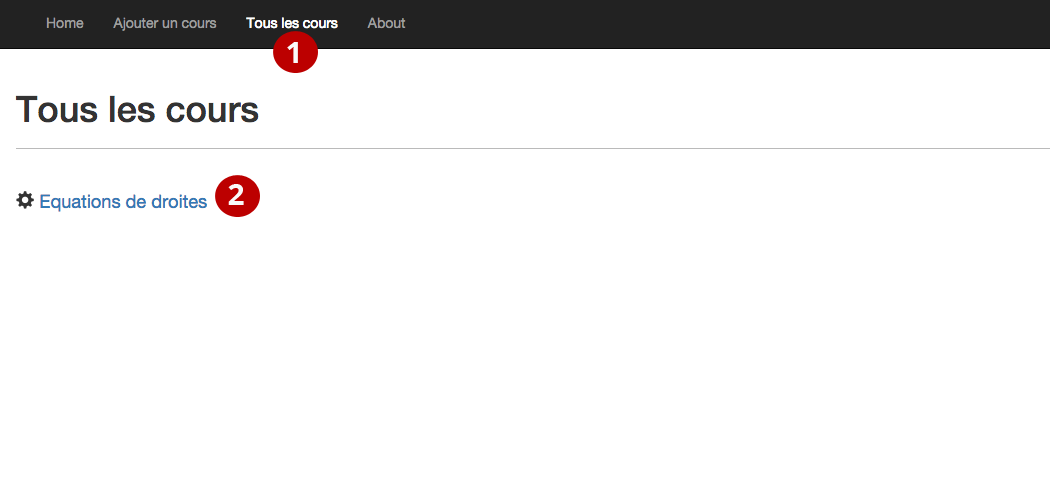
\includegraphics{all_courses.png}}
\caption{Tous les cours des professeurs}\end{figure}


\section{Les étudiants}
\label{functionalities:les-etudiants}
La plupart des fonctionnalités nécessitent que l'on soit connecté au site.


\subsection{Trouver un cours}
\label{functionalities:trouver-un-cours}
Tous les cours publiés sont consultables par les utilisateurs du site. S'ils se rendent sur la page ``Home'', les étudiants ont la liste du contenu mis à leur disposition. Ils peuvent afficher tous les cours (1), seulement leurs favoris (2), ou alors trouver un cours par thème (3). Grâce à cette organisation, chaque élève peut trouver rapidement et efficacement le cours qui répond à ses besoins. Lorsqu'un cours l'intéresse, il lui suffit de cliquer dessus (4) et il est alors redirigé sur la page de lecture du cours.
\begin{figure}[htbp]
\centering
\capstart

\scalebox{0.600000}{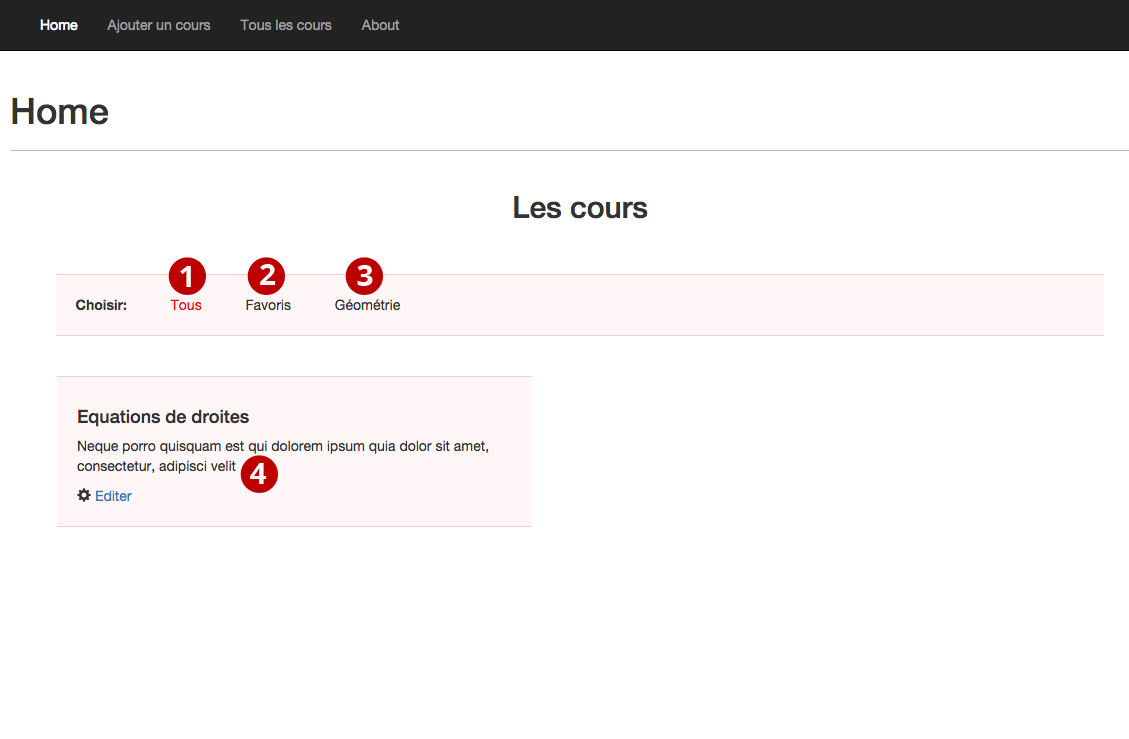
\includegraphics{home.png}}
\caption{Tous les cours}\end{figure}


\subsection{Lire un cours}
\label{functionalities:lire-un-cours}

\subsubsection{Les favoris}
\label{functionalities:les-favoris}
S'il apprécie particulièrement un cours, le trouve utile ou veut le retrouver facilement par la suite, l'étudiant peut l'ajouter en favoris, à l'instar des favoris d'un navigateur par exemple. Pour ce faire, il y a une étoile en haut de chaque page (1) de lecture d'un cours. Elle est d'abord vide, ce qui signifie que le cours n'appartient pas aux favoris de l'étudiant. Si l'on clique dessus, l'étoile devient pleine et signifie que le cours est ajouté à la liste de favoris. A l'inverse, l'élève peut évidemment retirer un favori de la même manière qu'il l'a ajouté. Sa liste de favoris peut être retrouvée sur la page d'accueil comme expliqué précédemment.


\subsubsection{La progression}
\label{functionalities:la-progression}
L'élève profite également d'un système d'indication de sa progression. L'objectif est de pouvoir faciliter son apprentissage à travers le cours, l'aider à suivre et identifier ses zones de faiblesse. En bas de chaque page d'un cours se situent deux boutons intitulés ``Compris'' et ``A relire'' (2). A la fin de sa lecture de la page, il est conseillé à l'élève de cliquer sur l'un des deux boutons. En effet, cela lui permettra ensuite de situer sa progression dans le cours. Basée sur les indications de l'utilisateur, une barre de progression en haut de la page (3) indique le nombre de pages comprises par rapport au nombre total de pages du cours. Quand il clique sur l'un des deux boutons, le lecteur est directement dirigé vers la page suivante et sa barre de progression est mise à jour. Il est évidemment possible de simplement cliquer sur ``Suivant'' (4) pour aller à la page suivante sans marquer la progression. Il y a aussi un bouton ``Précédent'' (5) pour se rendre à la page précédente.


\subsubsection{Télécharger le cours}
\label{functionalities:telecharger-le-cours}
Il est souvent pratique de pouvoir lire un cours sans connexion internet ou de pouvoir l'imprimer pour le lire sans ordinateur. C'est pourquoi il est possible d'obtenir le cours en version PDF ! Lorsque l'étudiant lit un cours, il peut voir un lien ``Télécharger le cours'' dans le menu à droite (6). Il suffit de cliquer sur le lien et après quelques instants l'on obtient le PDF.
\begin{figure}[htbp]
\centering
\capstart

\scalebox{0.600000}{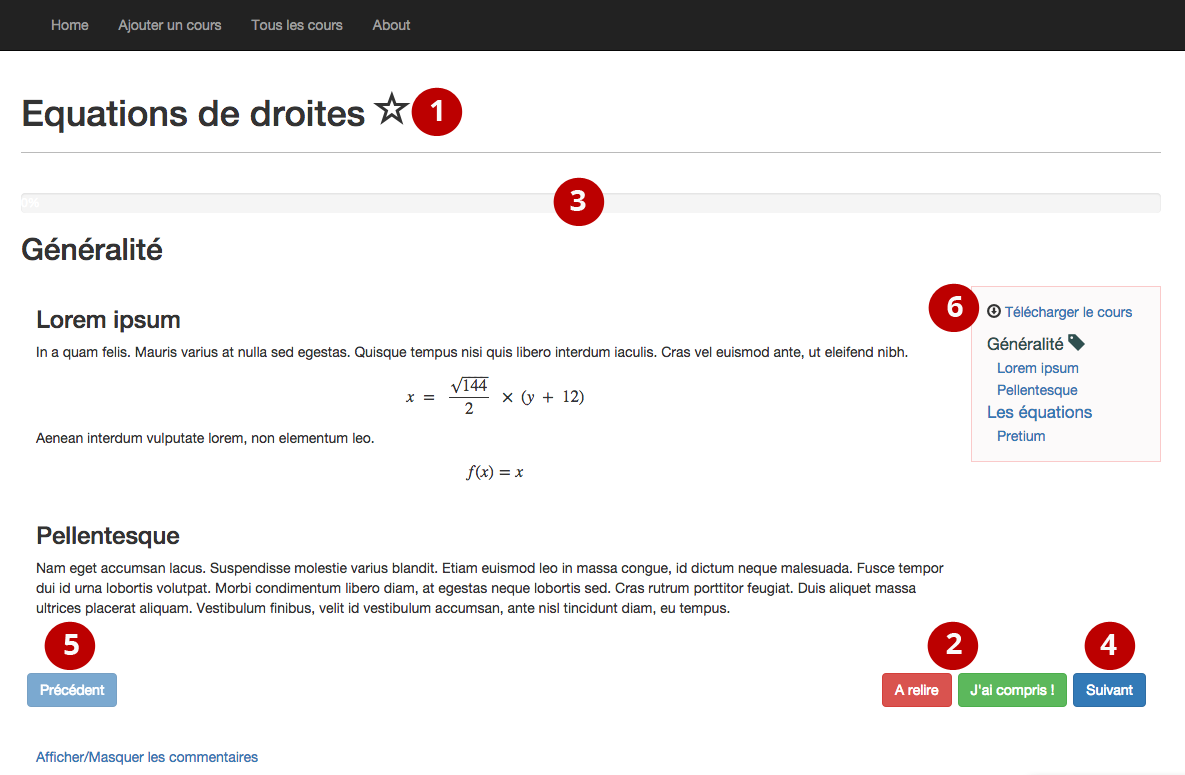
\includegraphics{view.png}}
\caption{Lire un cours}\end{figure}


\subsubsection{Les commentaires}
\label{functionalities:les-commentaires}
Chaque lecteur a la possibilité de commenter un cours, pour le complimenter, émettre une critique ou poser une question. En bas de chaque page du cours se trouve un lien ``Afficher/masquer les commentaires'' (1). Cela permet de montrer tous les commentaires ou de les cacher en cliquant dessus. Dans cette section, l'utilisateur voit chaque commentaire du cours avec son auteur et la date de publication (2). En dessous des commentaires se trouve une zone de texte (3) dans laquelle l'on peut écrire son propre commentaire. Au fur et à mesure que l'on tape son message, le commentaire s'affiche dans la liste (4), mais n'est pas encore envoyé. Une fois le texte rédigé, il faut le poster en cliquant sur le bouton ``Envoyer'' (5) pour qu'il soit instantanément visible par les autres lecteurs.
\begin{figure}[htbp]
\centering
\capstart

\scalebox{0.600000}{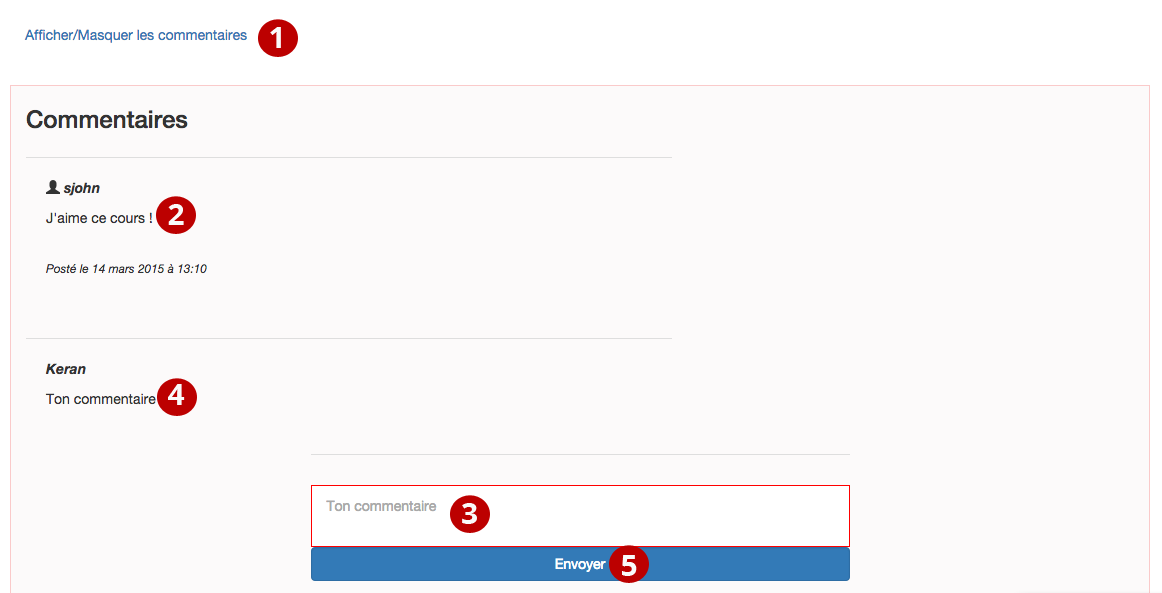
\includegraphics{comments.png}}
\caption{Les commentaires}\end{figure}


\chapter{Schémas}
\label{schemas::doc}\label{schemas:schemas}\begin{figure}[htbp]
\centering
\capstart

\scalebox{1.000000}{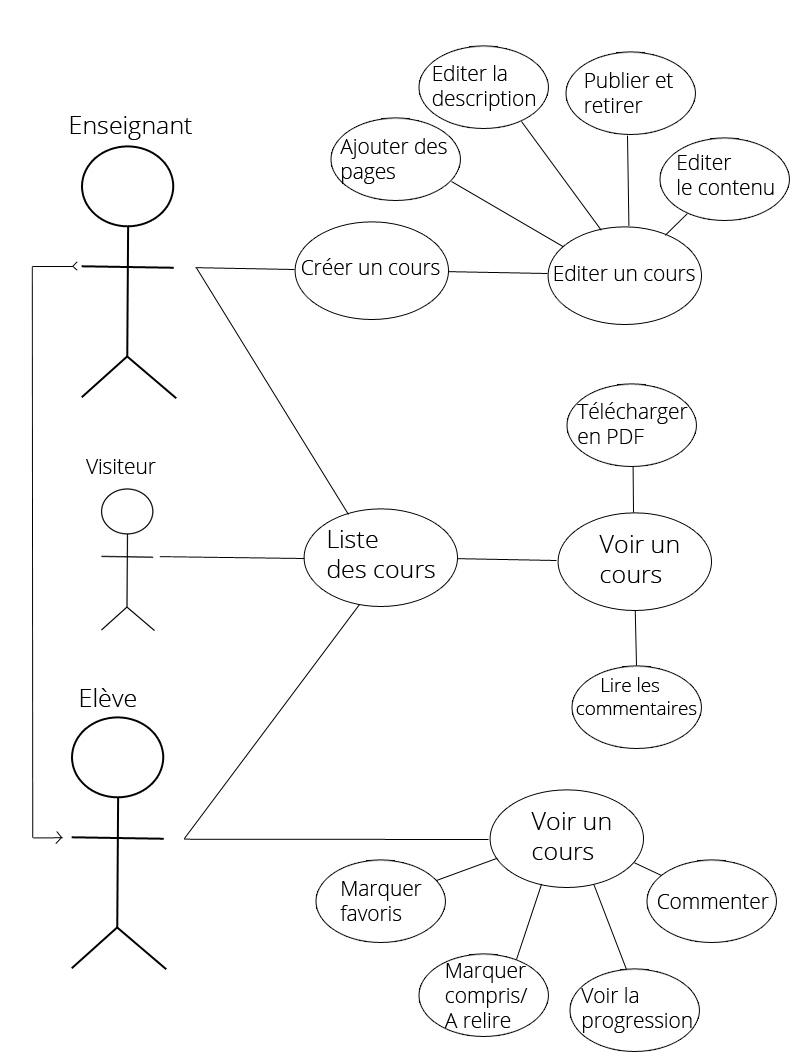
\includegraphics{use_cases.jpg}}
\caption{Cas d'utilisation}\end{figure}
\begin{figure}[htbp]
\centering
\capstart

\scalebox{0.800000}{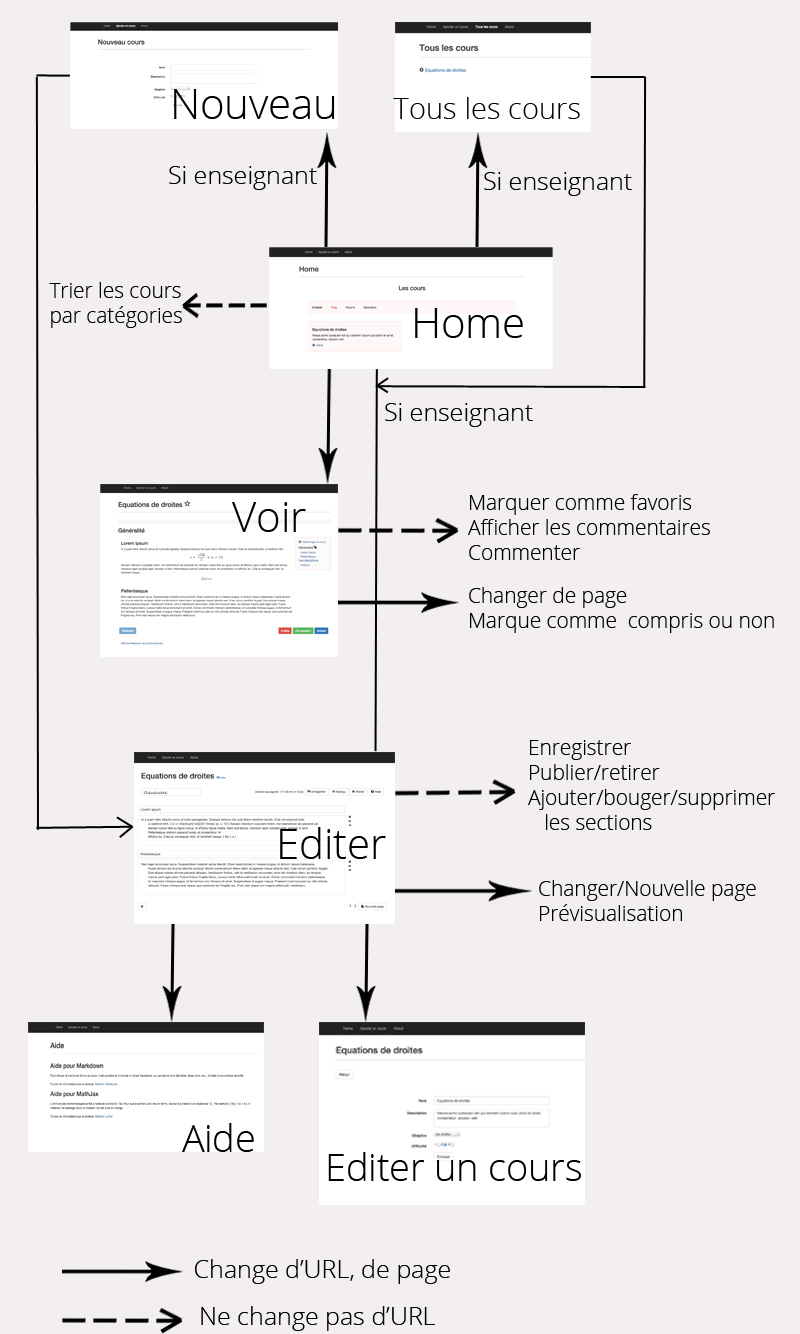
\includegraphics{navigation_schema.jpg}}
\caption{Schéma de navigation}\end{figure}


\chapter{Modèle relationnel}
\label{models::doc}\label{models:modele-relationnel}

\section{Introduction}
\label{models:introduction}
Une base de données est un outil permettant de stocker des données persistantes pour ensuite les réutiliser ou les conserver. Dans le domaine du web, on utilise principalement les bases de données relationnelles. Traditionnellement, elles se découpent en plusieurs tableaux que l'on appelle tables, contenant des colonnes et des lignes. On crée des tables pour représenter des entités, des cours par exemple, qui ont des attributs représentés par des colonnes. Ensuite, chaque ligne correspond à un enregistrement, c'est-à-dire une entité, un cours dans notre exemple. Une table a pratiquement toujours une colonne \code{id} qui est un nombre, un identifiant unique qui permet d'identifier un enregistrement parmi les autres de la table. On l'appelle \emph{clé primaire}. Ils servent aussi à créer des relations entre les tables, à lier un enregistrement à un autre. Nous verrons ces relations dans la construction du module de cours. Pour communiquer avec une base de données relationnelles, notamment chercher des enregistrements dans une table, créer ou mettre à jour un enregistrement, etc. l'on utilise le langage \emph{SQL}, \emph{Structured Query Language}.
\begin{figure}[htbp]
\centering
\capstart

\scalebox{0.900000}{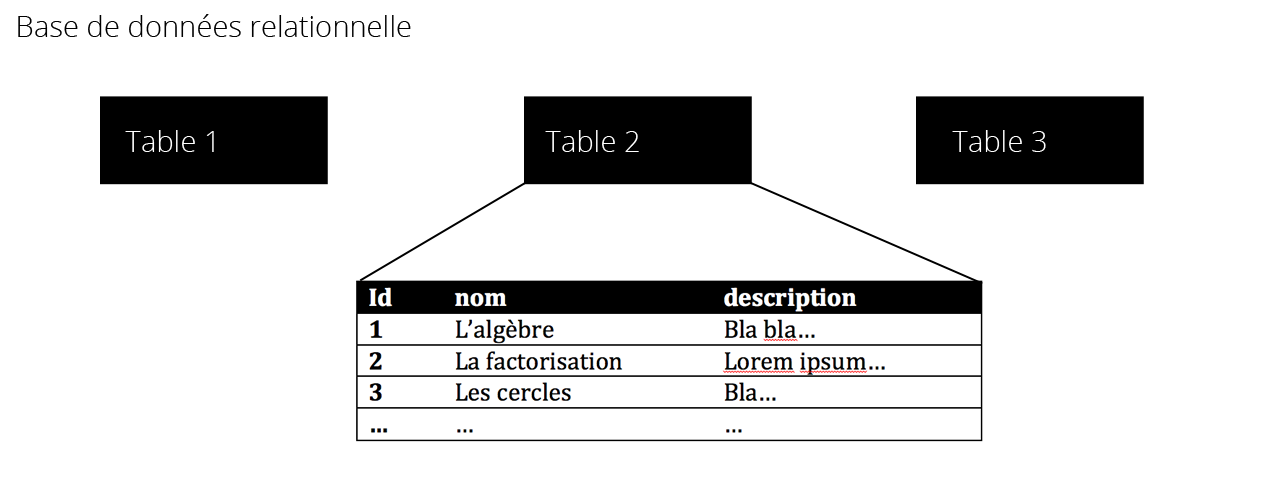
\includegraphics{bd.png}}
\caption{Schéma résumant une base de données relationnelle}\end{figure}

Le modèle relationnel est une modélisation de la base de données du site. Attardons-nous donc sur le modèle qui se cache derrière les fonctionnalités que nous voulons développer. Nous commencerons par le point central de la base de données: les tables et les relations qui concernent les cours et qui forment la majeure partie du modèle. Ensuite nous verrons les tables additionnelles qui complètent le modèle relationnel et ajoutent les fonctionnalités auxiliaires.

Il est important de savoir que Django fournit en tant que framework plusieurs outils facilitant le travail avec une base de données. Chaque table de notre \emph{BD} est représentée par ce que l'on appelle un modèle. C'est un simple fichier Python qui contient les informations pour construire la table. Dans le projet, les modèles sont regroupés dans le fichier \code{models.py}. Ce fichier permet à Django de générer les tables et ensuite de fournir une série de méthodes qui permettent de communiquer avec la \emph{BD} sans utiliser le langage SQL, qui est le seul langage que comprend une \emph{BD}. Django nous évite par conséquent d'apprendre un nouveau langage. Nous verrons ces méthodes plus tard dans les exemples d'utilisation.


\section{Les cours}
\label{models:les-cours}

\subsection{La structure}
\label{models:la-structure}\begin{figure}[htbp]
\centering
\capstart

\scalebox{0.900000}{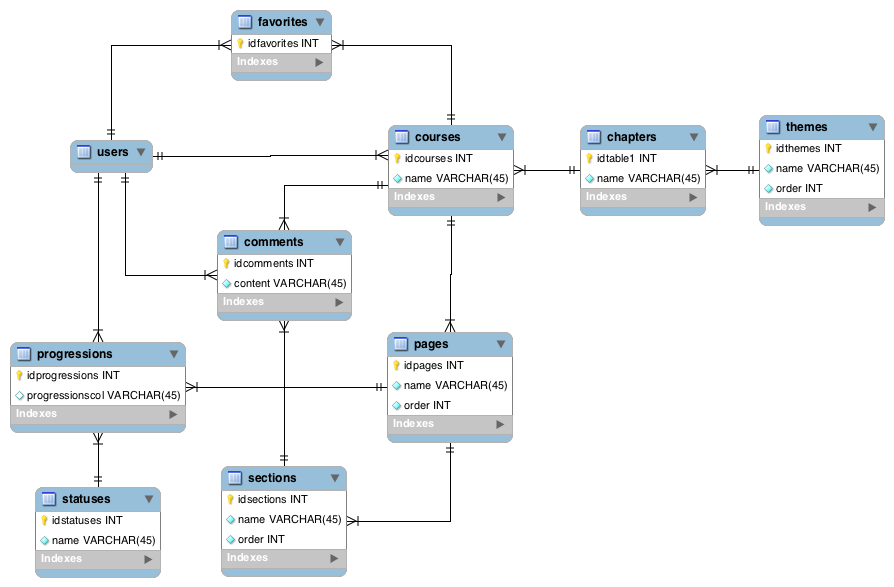
\includegraphics{uml_courses.png}}
\caption{Schéma de toutes les tables du modèle relationnel}\end{figure}

La structure des tables relationnelles reflète la structure que perçoit le rédacteur et cela facilite grandement la compréhension. Nous avons vu qu'un cours se compose de plusieurs pages. Elles-mêmes contiennent plusieurs sections, avec un titre et un contenu, que l'auteur peut éditer ou retirer à sa guise. C'est exactement la même chose dans la structure du modèle. Tout d'abord on trouve une table \code{courses} qui contient les informations de base que le professeur entre à la création du cours. Elle contient les colonnes suivantes: \code{name}, \code{description}, \code{difficulty}. Il reste le champ \code{chapter} que nous verrons plus tard. Ensuite, il y a la table \code{pages} avec la colonne \code{name}, \code{order} et \code{course\_id}. \code{name} est le titre de la page. \code{order} est un nombre qui permet de trier les pages d'un cours entre elles et de les réorganiser par la suite. \code{course\_id} indique la relation avec un cours. Elle contient l'\code{id} du cours auquel appartient la page. En effet, chaque page appartient à un cours et, vice-versa, un cours possède donc plusieurs pages. L'utilisation plus précise de cette relation est expliquée dans la partie suivante. Finalement, pour compléter l'ensemble, il reste la table \code{sections}. Elle possède les colonnes \code{name}, \code{content}, \code{order} et \code{page\_id}. On retrouve un titre et un contenu. Il y également l'ordre qui fonctionne comme pour les pages. \code{page\_id} indique la relation avec une page. Elle contient l'\code{id} de la page à laquelle appartient la section. Par conséquent, une section appartient à une page et une page possède plusieurs sections. A noter que ces trois tables ont également les champs \code{created\_at} et \code{updated\_at}. Elles enregistrent la date et l'heure de la création et la dernière mise à jour de l'entité. Pour résumer les relations qui lient les tables, un cours a plusieurs pages, et chacune des pages a plusieurs sections. Comme dit précédemment, l'on comprend facilement les relations en observant l'implémentation de l'interface de rédaction d'un cours.
\begin{figure}[htbp]
\centering
\capstart

\scalebox{0.800000}{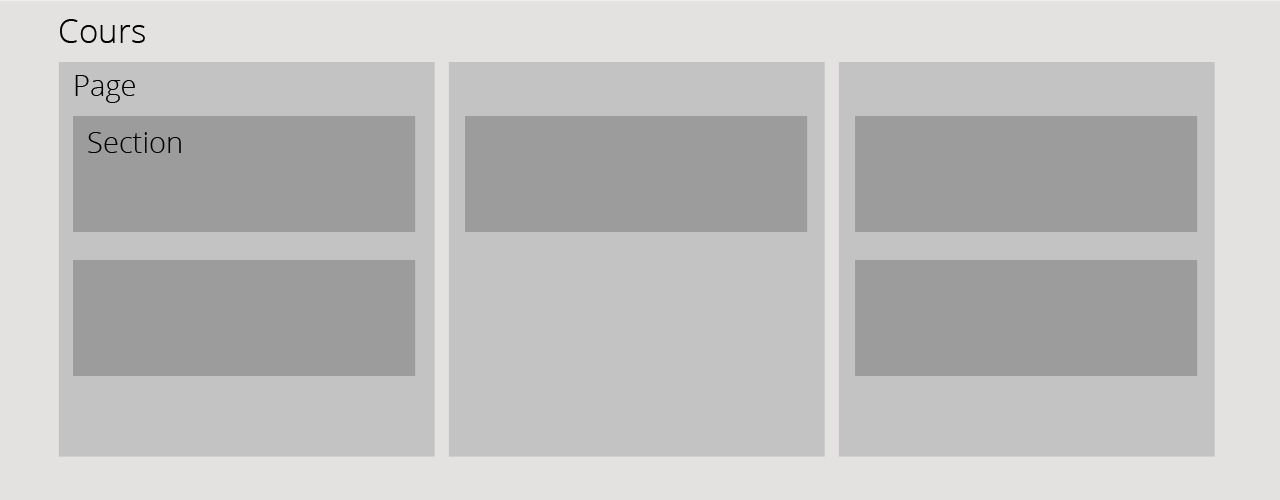
\includegraphics{schema_cours.png}}
\caption{Schéma qui résume les relations des tables courses, pages et sections}\end{figure}


\subsection{Utilisation}
\label{models:utilisation}
Tous les exemples d'opérations sur la base de données sont d'abord écrits avec les méthodes de Django puis en SQL pur. Une des particularités de Django pour sauvegarder des objets dans la base de données est qu'il fait appel à des formulaires. Ils sont nommés dans le code sous la forme de ....Form, comme \code{CourseForm} par exemple. On utilise aussi ces formulaires dans les vues pour générer les formulaires HTML que complètent les utilisateurs. Concrètement, ils permettent simplement de relier les données soumises par un utilisateur à nos modèles Django. Rappelons que dans Django les modèles sont la représentation des tables de la \emph{BD}. Par conséquent les formulaires Django servent à créer et à mettre à jour des enregistrements de la base de données via des formulaires HTML. Prenons un exemple pour bien se représenter le processus. Lorsqu'un utilisateur soumet un formulaire, le navigateur envoie les données au serveur sous la forme d'un dictionnaire: \code{\{"titre" : "La géométrie", "description" : "Bla bla"\}}. Ensuite, côté serveur, l'on récupère le dictionnaire et enregistre les données dans la \emph{BD} en utilisant un formulaire Django. Pour approfondir le concept des formulaires, il faut se rendre sur la \href{https://docs.djangoproject.com/fr/1.7/topics/forms/}{documentation Django} \footnote{
\href{https://docs.djangoproject.com/fr/1.7/topics/forms}{https://docs.djangoproject.com/fr/1.7/topics/forms}. Consulté le 20 décembre 14.
}.

Récupère tous les cours.

\begin{Verbatim}[commandchars=\\\{\}]
\PYG{c}{\PYGZsh{} api.py \PYGZhy{} TeacherCourseList}

\PYG{n}{Course}\PYG{o}{.}\PYG{n}{objects}\PYG{o}{.}\PYG{n}{all}\PYG{p}{(}\PYG{p}{)}
\end{Verbatim}

\begin{Verbatim}[commandchars=\\\{\}]
\PYG{k}{SELECT} \PYG{o}{*} \PYG{k}{FROM} \PYG{n}{courses}
\end{Verbatim}

Récupère tous les cours publiés ayant un thème particulier.

\begin{Verbatim}[commandchars=\\\{\}]
\PYG{c}{\PYGZsh{} api.py \PYGZhy{} CourseList}

\PYG{n}{Course}\PYG{o}{.}\PYG{n}{objects}\PYG{o}{.}\PYG{n}{filter}\PYG{p}{(}\PYG{n}{chapter\PYGZus{}\PYGZus{}theme\PYGZus{}\PYGZus{}name}\PYG{o}{=}\PYG{n}{request}\PYG{o}{.}\PYG{n}{GET}\PYG{p}{[}\PYG{l+s}{\PYGZsq{}}\PYG{l+s}{theme}\PYG{l+s}{\PYGZsq{}}\PYG{p}{]}\PYG{p}{,} \PYG{n}{published}\PYG{o}{=}\PYG{n+nb+bp}{True}\PYG{p}{)}
\end{Verbatim}

\begin{Verbatim}[commandchars=\\\{\}]
\PYG{c+c1}{\PYGZhy{}\PYGZhy{} SQL}

\PYG{k}{SELECT} \PYG{o}{*} \PYG{k}{FROM} \PYG{l+s+ss}{\PYGZdq{}courses\PYGZus{}course\PYGZdq{}} \PYG{k}{INNER} \PYG{k}{JOIN} \PYG{l+s+ss}{\PYGZdq{}teachers\PYGZus{}chapter\PYGZdq{}} \PYG{k}{ON} \PYG{p}{(} \PYG{l+s+ss}{\PYGZdq{}courses\PYGZus{}course\PYGZdq{}}\PYG{p}{.}\PYG{l+s+ss}{\PYGZdq{}chapter\PYGZus{}id\PYGZdq{}} \PYG{o}{=} \PYG{l+s+ss}{\PYGZdq{}teachers\PYGZus{}chapter\PYGZdq{}}\PYG{p}{.}\PYG{l+s+ss}{\PYGZdq{}id\PYGZdq{}} \PYG{p}{)}
\PYG{k}{INNER} \PYG{k}{JOIN} \PYG{l+s+ss}{\PYGZdq{}teachers\PYGZus{}theme\PYGZdq{}} \PYG{k}{ON} \PYG{p}{(} \PYG{l+s+ss}{\PYGZdq{}teachers\PYGZus{}chapter\PYGZdq{}}\PYG{p}{.}\PYG{l+s+ss}{\PYGZdq{}theme\PYGZus{}id\PYGZdq{}} \PYG{o}{=} \PYG{l+s+ss}{\PYGZdq{}teachers\PYGZus{}theme\PYGZdq{}}\PYG{p}{.}\PYG{l+s+ss}{\PYGZdq{}id\PYGZdq{}} \PYG{p}{)}
\PYG{k}{WHERE} \PYG{p}{(}\PYG{l+s+ss}{\PYGZdq{}teachers\PYGZus{}theme\PYGZdq{}}\PYG{p}{.}\PYG{l+s+ss}{\PYGZdq{}name\PYGZdq{}} \PYG{o}{=} \PYG{l+s+ss}{\PYGZdq{}Géométrie\PYGZdq{}} \PYG{k}{AND} \PYG{l+s+ss}{\PYGZdq{}courses\PYGZus{}course\PYGZdq{}}\PYG{p}{.}\PYG{l+s+ss}{\PYGZdq{}published\PYGZdq{}} \PYG{o}{=} \PYG{k}{True}\PYG{p}{)}
\end{Verbatim}

Crée un nouveau cours. On crée d'abord le cours, puis une page associée contenant une section vierge.

\begin{Verbatim}[commandchars=\\\{\}]
\PYG{c}{\PYGZsh{} api.py \PYGZhy{} CourseList}

\PYG{c}{\PYGZsh{} on utilise un formulaire (CourseForm)}
\PYG{c}{\PYGZsh{} request.data est un dictionnaire contenant les données soumises par l\PYGZsq{}utilisateur}
\PYG{c}{\PYGZsh{} ici les informations du cours}
\PYG{n}{course\PYGZus{}form} \PYG{o}{=} \PYG{n}{CourseForm}\PYG{p}{(}\PYG{n}{request}\PYG{o}{.}\PYG{n}{data}\PYG{p}{)}
\PYG{c}{\PYGZsh{} on vérifie si les informations sont présentes et valides}
\PYG{k}{if} \PYG{n}{course\PYGZus{}form}\PYG{o}{.}\PYG{n}{is\PYGZus{}valid}\PYG{p}{(}\PYG{p}{)}\PYG{p}{:}
    \PYG{c}{\PYGZsh{} on crée le cours}
    \PYG{n}{course} \PYG{o}{=} \PYG{n}{course\PYGZus{}form}\PYG{o}{.}\PYG{n}{save}\PYG{p}{(}\PYG{p}{)}
    \PYG{c}{\PYGZsh{} on crée la page associée}
    \PYG{n}{page} \PYG{o}{=} \PYG{n}{Page}\PYG{p}{(}\PYG{n}{name}\PYG{o}{=}\PYG{l+s}{\PYGZdq{}}\PYG{l+s}{Première page}\PYG{l+s}{\PYGZdq{}}\PYG{p}{,} \PYG{n}{order}\PYG{o}{=}\PYG{l+m+mi}{1}\PYG{p}{,} \PYG{n}{course\PYGZus{}id}\PYG{o}{=}\PYG{n}{course}\PYG{o}{.}\PYG{n}{id}\PYG{p}{)}
    \PYG{n}{page}\PYG{o}{.}\PYG{n}{save}\PYG{p}{(}\PYG{p}{)}
    \PYG{c}{\PYGZsh{} on crée une section associée à la page}
    \PYG{n}{page}\PYG{o}{.}\PYG{n}{sections}\PYG{o}{.}\PYG{n}{create}\PYG{p}{(}\PYG{n}{name}\PYG{o}{=}\PYG{l+s}{\PYGZdq{}}\PYG{l+s}{Première section}\PYG{l+s}{\PYGZdq{}}\PYG{p}{,} \PYG{n}{order}\PYG{o}{=}\PYG{l+m+mi}{1}\PYG{p}{)}
\end{Verbatim}

\begin{Verbatim}[commandchars=\\\{\}]
\PYG{c+c1}{\PYGZhy{}\PYGZhy{} SQL}

\PYG{c+c1}{\PYGZhy{}\PYGZhy{} on crée le cours}
\PYG{k}{INSERT} \PYG{k}{INTO} \PYG{n}{courses} \PYG{p}{(}\PYG{n}{name}\PYG{p}{,} \PYG{n}{description}\PYG{p}{,} \PYG{n}{difficulty}\PYG{p}{,} \PYG{n}{author\PYGZus{}id}\PYG{p}{,} \PYG{n}{chapter\PYGZus{}id}\PYG{p}{,} \PYG{n}{created\PYGZus{}at}\PYG{p}{,} \PYG{n}{updated\PYGZus{}at}\PYG{p}{)}
\PYG{k}{VALUES} \PYG{p}{(}\PYG{l+s+ss}{\PYGZdq{}L\PYGZsq{}algèbre\PYGZdq{}}\PYG{p}{,} \PYG{l+s+ss}{\PYGZdq{}Lorem ipsum...\PYGZdq{}}\PYG{p}{,} \PYG{l+m+mi}{3}\PYG{p}{,} \PYG{l+m+mi}{1}\PYG{p}{,} \PYG{l+m+mi}{1}\PYG{p}{,} \PYG{o}{*}\PYG{p}{,} \PYG{o}{*}\PYG{p}{)}
\PYG{c+c1}{\PYGZhy{}\PYGZhy{} =\PYGZgt{} ID du cours = 1}
\PYG{c+c1}{\PYGZhy{}\PYGZhy{} On crée la page associée}
\PYG{k}{INSERT} \PYG{k}{INTO} \PYG{n}{pages} \PYG{p}{(}\PYG{n}{name}\PYG{p}{,} \PYG{k}{order}\PYG{p}{,} \PYG{n}{course\PYGZus{}id}\PYG{p}{,} \PYG{n}{created\PYGZus{}at}\PYG{p}{,} \PYG{n}{updated\PYGZus{}at}\PYG{p}{)}
\PYG{k}{VALUES} \PYG{p}{(}\PYG{l+s+ss}{\PYGZdq{}Première page\PYGZdq{}}\PYG{p}{,} \PYG{l+m+mi}{1}\PYG{p}{,} \PYG{l+m+mi}{1}\PYG{p}{,} \PYG{o}{*}\PYG{p}{,} \PYG{o}{*}\PYG{p}{)}
\PYG{c+c1}{\PYGZhy{}\PYGZhy{} =\PYGZgt{} ID de la page = 1}
\PYG{c+c1}{\PYGZhy{}\PYGZhy{} on crée une section associée à la page}
\PYG{k}{INSERT} \PYG{k}{INTO} \PYG{n}{sections} \PYG{p}{(}\PYG{n}{name}\PYG{p}{,} \PYG{n}{content}\PYG{p}{,} \PYG{k}{order}\PYG{p}{,} \PYG{n}{page\PYGZus{}id}\PYG{p}{,} \PYG{n}{created\PYGZus{}at}\PYG{p}{,} \PYG{n}{updated\PYGZus{}at}\PYG{p}{)}
\PYG{k}{VALUES} \PYG{p}{(}\PYG{l+s+ss}{\PYGZdq{}Première section\PYGZdq{}}\PYG{p}{,} \PYG{l+s+ss}{\PYGZdq{}bla bla\PYGZdq{}}\PYG{p}{,} \PYG{l+m+mi}{1}\PYG{p}{,} \PYG{l+m+mi}{1}\PYG{p}{,} \PYG{o}{*}\PYG{p}{,} \PYG{o}{*}\PYG{p}{)}
\end{Verbatim}

Mettre à jour le contenu d'une page d'un cours. Le titre de la page, le titre et le contenu des sections vont être sauvegardés. Pour accomplir cette action, on commence par simplement enregistrer la page avec les nouvelles données. On utilise la même procédure que pour la création d'un cours. Remarquons simplement que dans \code{page\_form = PageForm(request.data, instance=page)}, l'on passe en paramètre la page provenant de la base de données, pour signaler à Django que l'enregistrement existe déjà. Ainsi Django ne crée pas une nouvelle page, mais met la nôtre à jour. Pour les sections, on itère d'abord sur le dictionnaire qui contient les données de toutes les sections de la page. Puis, pour chaque section, on accomplit la même procédure que pour une page.

\begin{Verbatim}[commandchars=\\\{\}]
\PYG{c}{\PYGZsh{} api.py \PYGZhy{} PageCourseDetail}

\PYG{c}{\PYGZsh{} Récupère la page à éditer}
\PYG{n}{page} \PYG{o}{=} \PYG{n}{Page}\PYG{o}{.}\PYG{n}{objects}\PYG{o}{.}\PYG{n}{get}\PYG{p}{(}\PYG{n+nb}{id}\PYG{o}{=}\PYG{n}{page\PYGZus{}id}\PYG{p}{)}
\PYG{c}{\PYGZsh{} On utilise un formulaire (PageForm)}
\PYG{c}{\PYGZsh{} request.data est un dictionnaire contenant les données soumises par l\PYGZsq{}utilisateur}
\PYG{c}{\PYGZsh{} ici le contenu de la page}
\PYG{n}{page\PYGZus{}form} \PYG{o}{=} \PYG{n}{PageForm}\PYG{p}{(}\PYG{n}{request}\PYG{o}{.}\PYG{n}{data}\PYG{p}{,} \PYG{n}{instance}\PYG{o}{=}\PYG{n}{page}\PYG{p}{)}
\PYG{c}{\PYGZsh{} On vérifie si les informations sont présentes et valides}
\PYG{k}{if} \PYG{n}{page\PYGZus{}form}\PYG{o}{.}\PYG{n}{is\PYGZus{}valid}\PYG{p}{(}\PYG{p}{)}\PYG{p}{:}
    \PYG{c}{\PYGZsh{} On enregistre la page \PYGZhy{} sauvegarde le titre}
    \PYG{n}{page\PYGZus{}form}\PYG{o}{.}\PYG{n}{save}\PYG{p}{(}\PYG{p}{)}
\PYG{c}{\PYGZsh{} On récupère le dictionnaire contenant les données des sections}
\PYG{n}{sections\PYGZus{}params} \PYG{o}{=} \PYG{n}{request}\PYG{o}{.}\PYG{n}{data}\PYG{p}{[}\PYG{l+s}{\PYGZsq{}}\PYG{l+s}{sections}\PYG{l+s}{\PYGZsq{}}\PYG{p}{]}
\PYG{c}{\PYGZsh{} On fait une boucle pour chaque section}
\PYG{k}{for} \PYG{n}{section\PYGZus{}params} \PYG{o+ow}{in} \PYG{n}{sections\PYGZus{}params}\PYG{p}{:}
    \PYG{c}{\PYGZsh{} On récupère la section}
    \PYG{n}{section} \PYG{o}{=} \PYG{n}{Section}\PYG{o}{.}\PYG{n}{objects}\PYG{o}{.}\PYG{n}{get}\PYG{p}{(}\PYG{n+nb}{id}\PYG{o}{=}\PYG{n}{section\PYGZus{}params}\PYG{p}{[}\PYG{l+s}{\PYGZsq{}}\PYG{l+s}{id}\PYG{l+s}{\PYGZsq{}}\PYG{p}{]}\PYG{p}{)}
    \PYG{c}{\PYGZsh{} On utilise un formulaire (SectionForm)}
    \PYG{c}{\PYGZsh{} section\PYGZus{}params est un dictionnaire contenant le titre et le contenu de la section}
    \PYG{n}{section\PYGZus{}form} \PYG{o}{=} \PYG{n}{SectionForm}\PYG{p}{(}\PYG{n}{section\PYGZus{}params}\PYG{p}{,} \PYG{n}{instance}\PYG{o}{=}\PYG{n}{section}\PYG{p}{)}
    \PYG{c}{\PYGZsh{} On vérifie si les informations sont présentes et valides}
    \PYG{k}{if} \PYG{n}{section\PYGZus{}form}\PYG{o}{.}\PYG{n}{is\PYGZus{}valid}\PYG{p}{(}\PYG{p}{)}\PYG{p}{:}
        \PYG{c}{\PYGZsh{} On enregistre la section}
        \PYG{n}{section\PYGZus{}form}\PYG{o}{.}\PYG{n}{save}\PYG{p}{(}\PYG{p}{)}
\end{Verbatim}

\begin{Verbatim}[commandchars=\\\{\}]
\PYG{c+c1}{\PYGZhy{}\PYGZhy{} SQL}

\PYG{c+c1}{\PYGZhy{}\PYGZhy{} Récupère la page à éditer}
\PYG{k}{SELECT} \PYG{o}{*} \PYG{k}{FROM} \PYG{n}{pages} \PYG{k}{WHERE} \PYG{n}{id} \PYG{o}{=} \PYG{l+m+mi}{1}
\PYG{c+c1}{\PYGZhy{}\PYGZhy{} On enregistre la page}
\PYG{k}{UPDATE} \PYG{n}{pages} \PYG{k}{SET} \PYG{n}{name} \PYG{o}{=} \PYG{l+s+ss}{\PYGZdq{}Nouveau titre\PYGZdq{}} \PYG{k}{WHERE} \PYG{n}{id} \PYG{o}{=} \PYG{l+m+mi}{1}
\PYG{c+c1}{\PYGZhy{}\PYGZhy{} On enregistre la section}
\PYG{k}{UPDATE} \PYG{n}{sections} \PYG{k}{SET} \PYG{n}{name} \PYG{o}{=} \PYG{l+s+ss}{\PYGZdq{}Nouveau titre\PYGZdq{}}\PYG{p}{,} \PYG{l+s+ss}{\PYGZdq{}content\PYGZdq{}} \PYG{o}{=} \PYG{l+s+ss}{\PYGZdq{}Lorem ispum\PYGZdq{}} \PYG{k}{WHERE} \PYG{n}{id} \PYG{o}{=} \PYG{l+m+mi}{1}
\end{Verbatim}


\section{Les chapitres}
\label{models:les-chapitres}
Pour pouvoir organiser le contenu du site, chaque cours est associé à un chapitre. Deux tables servent cet objectif. Tout d'abord il y a la table \code{themes} avec un champs \code{name}. Il y a également la table \code{chapters} avec un champ \code{name} et \code{theme\_id}. \code{theme\_id} associe chaque chapitre à un thème. Ensuite la table \code{courses} a un champ \code{chapter\_id}. Celui-ci contient l'\code{id} d'un chapitre. Il relie chaque cours à un chapitre et par conséquent à un thème. Par exemple, il peut y avoir un cours sur les tangentes. On le placerait dans le chapitre ``les cercles'' et le chapitre se trouverait lui-même dans le thème ``Géométrie''. On peut légitiment se demander pourquoi ces deux niveaux et ces deux tables ? Le système est construit afin de laisser une plus grande souplesse et liberté pour organiser le contenu. En effet, imaginons qu'il y ait 10, 20, 30 ou plus chapitres, comment s'y retrouver ? La solution est de les regrouper sous une idée plus générale, et c'est précisément le rôle de la table \code{themes}.


\section{Les commentaires}
\label{models:les-commentaires}
La table \code{course\_comments} permet aux lecteurs du site de poster un commentaire sur un cours. La table contient un champ \code{content}, \code{user\_id} et \code{course\_id}. Chaque commentaire appartient donc à un utilisateur et à un cours.


\section{La progression}
\label{models:la-progression}
L'utilisateur a la possibilité de marquer sa progression quand il lit un cours. Voyons comment cette fonctionnalité se traduit au niveau du modèle relationnel. \code{progressions} est la table principale. Elle contient les colonnes \code{page\_id}, \code{user\_id} et \code{status\_id}. En somme, elle ne contient que des relations. L'idée principale est la suivante; lorsqu'un utilisateur a lu une page d'un cours, on lui propose de choisir s'il a compris ou souhaite relire la page. Le champ \code{user\_id} enregistre quel utilisateur indique sa progression et le champ \code{page\_id} indique quelle page est concernée. Finalement, l'attribut \code{status\_id} associe la progression à une table \code{statuses}. Celle-ci contient le nom que peut avoir une progression. Il y a deux statuts: ``Compris'' et ``A relire''. Pour résumer, lorsque que l'on crée une progression dans notre base de données, l'on sait qu'un certain utilisateur a ``compris'' ou souhaite ``relire'' une page particulière. L'exemple qui suit montre comment l'on enregistre une progression concrètement.

\begin{Verbatim}[commandchars=\\\{\}]
\PYG{c}{\PYGZsh{} api.py \PYGZhy{} CoursePageProgress}

\PYG{c}{\PYGZsh{} On récupère l\PYGZsq{}utilisateur connecté au site}
\PYG{n}{user} \PYG{o}{=} \PYG{n}{request}\PYG{o}{.}\PYG{n}{user}
\PYG{c}{\PYGZsh{} On récupère la page concernée}
\PYG{n}{page} \PYG{o}{=} \PYG{n}{Page}\PYG{o}{.}\PYG{n}{objects}\PYG{o}{.}\PYG{n}{get}\PYG{p}{(}\PYG{n+nb}{id}\PYG{o}{=}\PYG{n}{pk}\PYG{p}{)}

\PYG{c}{\PYGZsh{} request.data est un dictionnaire contenant les données soumises par l\PYGZsq{}utilisateur}
\PYG{c}{\PYGZsh{} ici, si l\PYGZsq{}utilisateur a compris ou non la page}
\PYG{c}{\PYGZsh{} On choisit le statut en fonction}
\PYG{k}{if} \PYG{n}{request}\PYG{o}{.}\PYG{n}{data}\PYG{p}{[}\PYG{l+s}{\PYGZsq{}}\PYG{l+s}{is\PYGZus{}done}\PYG{l+s}{\PYGZsq{}}\PYG{p}{]} \PYG{o}{==} \PYG{n+nb+bp}{True}\PYG{p}{:}
    \PYG{n}{status} \PYG{o}{=} \PYG{n}{Status}\PYG{o}{.}\PYG{n}{objects}\PYG{o}{.}\PYG{n}{get}\PYG{p}{(}\PYG{n}{name}\PYG{o}{=}\PYG{l+s}{\PYGZdq{}}\PYG{l+s}{Compris}\PYG{l+s}{\PYGZdq{}}\PYG{p}{)}
\PYG{k}{else}\PYG{p}{:}
    \PYG{n}{status} \PYG{o}{=} \PYG{n}{Status}\PYG{o}{.}\PYG{n}{objects}\PYG{o}{.}\PYG{n}{get}\PYG{p}{(}\PYG{n}{name}\PYG{o}{=}\PYG{l+s}{\PYGZdq{}}\PYG{l+s}{Relire}\PYG{l+s}{\PYGZdq{}}\PYG{p}{)}

\PYG{c}{\PYGZsh{} Si l\PYGZsq{}utilisateur n\PYGZsq{}a pas encore marqué sa progression sur cette page}
\PYG{k}{if} \PYG{o+ow}{not} \PYG{n}{page}\PYG{o}{.}\PYG{n}{state}\PYG{p}{(}\PYG{n}{user}\PYG{p}{)}\PYG{p}{:}
    \PYG{c}{\PYGZsh{} On crée une progression avec la page, le statut et l\PYGZsq{}utilisateur}
    \PYG{n}{page}\PYG{o}{.}\PYG{n}{progression\PYGZus{}set}\PYG{o}{.}\PYG{n}{create}\PYG{p}{(}\PYG{n}{status}\PYG{o}{=}\PYG{n}{status}\PYG{p}{,} \PYG{n}{user}\PYG{o}{=}\PYG{n}{user}\PYG{p}{)}
\PYG{c}{\PYGZsh{} si l\PYGZsq{}utilisateur a déjà marqué sa progression sur cette page}
\PYG{k}{else}\PYG{p}{:}
    \PYG{c}{\PYGZsh{} On récupère sa progression}
    \PYG{n}{progression} \PYG{o}{=} \PYG{n}{page}\PYG{o}{.}\PYG{n}{progression\PYGZus{}set}\PYG{o}{.}\PYG{n}{get}\PYG{p}{(}\PYG{n}{user}\PYG{o}{=}\PYG{n}{user}\PYG{p}{)}
    \PYG{c}{\PYGZsh{} On met à jour avec le nouveau statut}
    \PYG{n}{progression}\PYG{o}{.}\PYG{n}{status} \PYG{o}{=} \PYG{n}{status}
    \PYG{n}{progression}\PYG{o}{.}\PYG{n}{save}\PYG{p}{(}\PYG{p}{)}
\end{Verbatim}

\begin{Verbatim}[commandchars=\\\{\}]
\PYG{c+c1}{\PYGZhy{}\PYGZhy{} SQL}

\PYG{c+c1}{\PYGZhy{}\PYGZhy{} Récupère la page à éditer}
\PYG{k}{SELECT} \PYG{o}{*} \PYG{k}{FROM} \PYG{n}{pages} \PYG{k}{WHERE} \PYG{n}{id} \PYG{o}{=} \PYG{l+m+mi}{1}
\PYG{c+c1}{\PYGZhy{}\PYGZhy{} =\PYGZgt{} ID de la page = 1}
\PYG{c+c1}{\PYGZhy{}\PYGZhy{} Récupère le statut}
\PYG{k}{SELECT} \PYG{o}{*} \PYG{k}{FROM} \PYG{n}{statuses} \PYG{k}{WHERE} \PYG{n}{name} \PYG{o}{=} \PYG{l+s+ss}{\PYGZdq{}Compris\PYGZdq{}}
\PYG{c+c1}{\PYGZhy{}\PYGZhy{} =\PYGZgt{} ID du statut = 1}
\PYG{c+c1}{\PYGZhy{}\PYGZhy{} Crée une progression}
\PYG{k}{INSERT} \PYG{k}{INTO} \PYG{l+s+ss}{\PYGZdq{}progressions\PYGZdq{}} \PYG{p}{(}\PYG{l+s+ss}{\PYGZdq{}page\PYGZus{}id\PYGZdq{}}\PYG{p}{,} \PYG{l+s+ss}{\PYGZdq{}status\PYGZus{}id\PYGZdq{}}\PYG{p}{,} \PYG{l+s+ss}{\PYGZdq{}user\PYGZus{}id\PYGZdq{}}\PYG{p}{,} \PYG{l+s+ss}{\PYGZdq{}created\PYGZus{}at\PYGZdq{}}\PYG{p}{,} \PYG{l+s+ss}{\PYGZdq{}updated\PYGZus{}at\PYGZdq{}}\PYG{p}{)}
\PYG{k}{VALUES} \PYG{p}{(}\PYG{l+m+mi}{1}\PYG{p}{,} \PYG{l+m+mi}{1}\PYG{p}{,} \PYG{l+m+mi}{1}\PYG{p}{,} \PYG{o}{*}\PYG{p}{,} \PYG{o}{*}\PYG{p}{)}
\PYG{c+c1}{\PYGZhy{}\PYGZhy{} Met à jour une progression}
\PYG{k}{UPDATE} \PYG{l+s+ss}{\PYGZdq{}progressions\PYGZdq{}} \PYG{k}{SET} \PYG{n}{status\PYGZus{}id} \PYG{o}{=} \PYG{l+m+mi}{1} \PYG{k}{WHERE} \PYG{n}{id} \PYG{o}{=} \PYG{l+m+mi}{1}
\end{Verbatim}


\chapter{RestLess}
\label{restless::doc}\label{restless:restless}

\section{Présentation}
\label{restless:presentation}
\href{https://github.com/dobarkod/django-restless}{RestLess} \footnote{
\href{https://github.com/dobarkod/django-restless}{https://github.com/dobarkod/django-restless}. Consulté le 4 janvier 15.
} est un set d'outils permettant de faciliter l'implémentation d'une API JSON dans Django. Il a l'avantage d'être léger et facile à utiliser comme nous le verrons par la suite. Une API, Application Programming Interface, est basiquement une application qui offre des services accessibles par une autre application. Le JSON est un format de données dans le style d'un dictionnaire \code{\{"nom" : "Keran", "prenom" : "Kocher"\}}. On appelle donc une API JSON une application qui fournit des données en format JSON. Concrètement, il s'agit d'une série d'URL qui fournissent le contenu de différentes tables de la BD en format JSON. Quand on se rend sur une de ces URL, on ne voit pas une page HTML, mais simplement un dictionnaire de données. Sur notre site web rendez-vous sur \code{http://webmath.com/courses/api/themes} pour voir à quoi ressemble la page.

Dans la présentation d'AngularJS, nous avons vu que le framework n'est pas capable de communiquer directement avec une base de données. C'est une limitation de JavaScript, qui s'exécute du côté du client dans notre cas. Pour palier à ce problème, on utilise un langage intermédiaire qui est capable de communiquer avec une BD et qui s'exécute côté serveur, c'est le cas de Python et son framework Django. On va donc construire une API avec Django. API à laquelle notre application AngularJS va pouvoir accéder. Dans les fait, Django va chercher les données dans la base de données, les transforme en format JSON puis les sert. Il suffit ensuite avec AngularJS d'accéder à l'URL correspondante et l'on dispose ensuite des données que l'on peut utiliser à sa guise dans nos vues AngularJS.


\section{Les vues génériques}
\label{restless:les-vues-generiques}
Lorsqu'on développe une application web, cela donne souvent un code redondant, répétitif. En effet, quand on crée des fonctionnalités, il s'agit généralement d'une table dans la base de données, avec laquelle on communique pour ajouter ou modifier des données. Et ces interactions se ressemblent dans la plupart des cas. On parle généralement du CRUD: create, read, update and delete, en français créer, lire, mettre à jour et supprimer. On a une table et on veut accomplir les opérations CRUD dessus. Pour ce faire, l'on a une série d'URL qui exécutent différentes actions. Prenons l'exemple de la création d'un blog tout à fait typique. On va créer une table \code{articles}, et implémenter les actions suivantes: on veut pouvoir afficher tous les articles, ou n'en afficher qu'un seul, ajouter un nouvel article, le mettre à jour ou le supprimer. Ainsi, avec ces quatre opérations, l'on peut disposer d'un blog complet et fonctionnel. Pour beaucoup de fonctionnalités, il s'agit d'effectuer toujours ces mêmes opérations classiques; un autre exemple serait un système de commentaires. Pour programmer ces outils basiques et conventionnels, deux moyens sont à notre disposition dans Django. D'abord, l'on peut programmer les opérations de A à Z. Avec Django, il s'agit basiquement de créer une URL et de lui assigner une fonction qui s'occupe de communiquer avec la base de données, et qui retourne une page HTML. Si l'on utilise cette méthode, on risque de devoir programmer souvent le même code au fil du développement et de perdre du temps. Ci-dessous le code pour afficher tous les articles avec la première méthode.

\begin{Verbatim}[commandchars=\\\{\}]
\PYG{c}{\PYGZsh{} urls.py \PYGZhy{} fichier qui gère les URL du site}

\PYG{k+kn}{from} \PYG{n+nn}{django.conf.urls} \PYG{k+kn}{import} \PYG{n}{patterns}\PYG{p}{,} \PYG{n}{url}\PYG{p}{,} \PYG{n}{include}

\PYG{k+kn}{from} \PYG{n+nn}{courses} \PYG{k+kn}{import} \PYG{n}{views}

\PYG{c}{\PYGZsh{} On crée une URL /articles qui utilise la fonction index \PYGZhy{} voir fichier views.py}
\PYG{n}{urlpatterns} \PYG{o}{=} \PYG{n}{patterns}\PYG{p}{(}\PYG{l+s}{\PYGZsq{}}\PYG{l+s}{\PYGZsq{}}\PYG{p}{,}
    \PYG{n}{url}\PYG{p}{(}\PYG{l+s}{r\PYGZsq{}}\PYG{l+s}{\PYGZca{}articles\PYGZdl{}}\PYG{l+s}{\PYGZsq{}}\PYG{p}{,} \PYG{n}{views}\PYG{o}{.}\PYG{n}{index}\PYG{p}{)}\PYG{p}{,}
\PYG{p}{)}

\PYG{c}{\PYGZsh{} views.py \PYGZhy{} fichier qui contient les fonctions liées aux URL}
\PYG{c}{\PYGZsh{} = vue ou contrôleur}

\PYG{k+kn}{from} \PYG{n+nn}{django.shortcuts} \PYG{k+kn}{import} \PYG{n}{render}

\PYG{c}{\PYGZsh{} Fonction reliée à /articles}
\PYG{k}{def} \PYG{n+nf}{index}\PYG{p}{(}\PYG{n}{request}\PYG{p}{)}\PYG{p}{:}
    \PYG{c}{\PYGZsh{} Récupère tous les articles de la BD (fait appelle au modèle Article)}
    \PYG{n}{articles} \PYG{o}{=} \PYG{n}{Article}\PYG{o}{.}\PYG{n}{objects}\PYG{o}{.}\PYG{n}{all}\PYG{p}{(}\PYG{p}{)}
    \PYG{c}{\PYGZsh{} Retourne le code HTML en utilisant le ficher courses.html}
    \PYG{k}{return} \PYG{n}{render}\PYG{p}{(}\PYG{n}{request}\PYG{p}{,} \PYG{l+s}{\PYGZdq{}}\PYG{l+s}{courses/courses.html}\PYG{l+s}{\PYGZdq{}}\PYG{p}{,} \PYG{n+nb}{locals}\PYG{p}{(}\PYG{p}{)}\PYG{p}{)}
\end{Verbatim}

La deuxième méthode consiste à utiliser les vues génériques. Ce sont des classes dans Django contenant les opérations conventionnelles déjà écrites. Il nous suffit donc de créer notre propre classe qui hérite d'une vue générique Django et d'ensuite la relier à notre URL, comme on le faisait précédemment avec la fonction. Pourquoi créer une classe et ne pas utiliser directement les classes Django ? On agit ainsi tout simplement pour pouvoir personnaliser la classe. Il faut déjà obligatoirement spécifier le modèle que doit utiliser la classe, par exemple pour savoir quels enregistrements elle doit aller récupérer. Regardons la même fonctionnalité qu'avant, mais écrite avec les vues génériques.

\begin{Verbatim}[commandchars=\\\{\}]
\PYG{c}{\PYGZsh{} urls.py \PYGZhy{} fichier qui gère les URL du site}

\PYG{k+kn}{from} \PYG{n+nn}{django.conf.urls} \PYG{k+kn}{import} \PYG{n}{patterns}\PYG{p}{,} \PYG{n}{url}\PYG{p}{,} \PYG{n}{include}

\PYG{k+kn}{from} \PYG{n+nn}{courses.views} \PYG{k+kn}{import} \PYG{n}{ArticlesList}

\PYG{c}{\PYGZsh{} On crée une URL /articles qui utilise la vue générique ArticlesList \PYGZhy{} voir fichier views.py}
\PYG{n}{urlpatterns} \PYG{o}{=} \PYG{n}{patterns}\PYG{p}{(}\PYG{l+s}{\PYGZsq{}}\PYG{l+s}{\PYGZsq{}}\PYG{p}{,}
    \PYG{n}{url}\PYG{p}{(}\PYG{l+s}{r\PYGZsq{}}\PYG{l+s}{\PYGZca{}articles\PYGZdl{}}\PYG{l+s}{\PYGZsq{}}\PYG{p}{,} \PYG{n}{ArticlesList}\PYG{o}{.}\PYG{n}{as\PYGZus{}view}\PYG{p}{(}\PYG{p}{)}\PYG{p}{)}\PYG{p}{,}
\PYG{p}{)}

\PYG{c}{\PYGZsh{} views.py \PYGZhy{} fichier qui contient les fonctions liées aux URL}
\PYG{c}{\PYGZsh{} = vue ou contrôleur}

\PYG{k+kn}{from} \PYG{n+nn}{django.views.generic} \PYG{k+kn}{import} \PYG{n}{ListView}

\PYG{c}{\PYGZsh{} La classe générique reliée à /articles}
\PYG{c}{\PYGZsh{} Hérite de ListView, classe provenant de Django}
\PYG{k}{class} \PYG{n+nc}{ArticlesList}\PYG{p}{(}\PYG{n}{ListView}\PYG{p}{)}\PYG{p}{:}

    \PYG{c}{\PYGZsh{} On spécifie le modèle à utiliser}
    \PYG{n}{model} \PYG{o}{=} \PYG{n}{Article}
\end{Verbatim}

Avec la seconde méthode, le code est plus concis. L'exemple montre comment générer la liste des articles, mais il existe une vue générique pour chaque opération CRUD. Il est encore possible de personnaliser notre classe \code{ArticlesList} avec des options ou en surchargeant les méthodes. En revanche, si notre fonctionnalité a des besoins spécifiques qui s'éloignent trop de la convention, les vues génériques ne sont plus adaptées, car leur personnalisation a évidemment des limites. Dans ces cas-ci, on retourne à la première méthode. Toutes les explications et options des vues génériques se trouvent dans la \href{https://docs.djangoproject.com/fr/1.7/topics/class-based-views/generic-display/}{documentation Django}  \footnote{
\href{https://docs.djangoproject.com/fr/1.7/topics/class-based-views/generic-display}{https://docs.djangoproject.com/fr/1.7/topics/class-based-views/generic-display}. Consulté le 4 janvier 15.
}.


\section{Fonctionnement de RestLess}
\label{restless:fonctionnement-de-restless}
Nous avons étudié ce qu'étaient les vues génériques dans Django, parce que RestLess se base exclusivement sur ce concept pour construire une API JSON. En fait, RestLess fournit également des vues génériques qui sont des dérivées des classes Django. Les classes de RestLess font en effet exactement le même travail que celle de Django, à la différence qu'elles travaillent avec le format JSON. Ainsi, on peut construire facilement et rapidement notre API, en économisant du code et du temps. En revanche, Django possède beaucoup de vues génériques et RestLess n'offre que les plus utiles. Avant de nous intéresser aux classes que nous pouvons utiliser avec RestLess, il nous faut d'abord voir les différents types de requêtes qui existent dans le monde du web.


\subsection{HTTP}
\label{restless:http}
HTTP est l'abréviation de \emph{HyperText Transfer Protocol} qui veut dire \emph{protocole de transfert hypertexte}. Ce protocole est utilisé sur internet pour la communication entre un client et un serveur. Le serveur est un ordinateur dont le rôle est de fournir le contenu désiré d'un site web. Le client est un navigateur utilisé par une personne qui navigue sur un site web. Lorsqu'un utilisateur visite une page, le navigateur demande au serveur la page HTML correspondante et ensuite il l'affiche à l'utilisateur. Pour établir le transfert de données, on utilise donc HTTP. Quand le client demande une information au serveur, on appelle cela une requête HTTP. Il y a plusieurs types de requêtes HTTP. Nous avons vu que le serveur envoie des données au client, mais le contraire est aussi vrai. Le client peut envoyer des données au serveur, quand il soumet un formulaire HTML par exemple. Ces différentes requêtes, formulées par un navigateur qui est le client, servent en général à agir sur une ressource en permettant notamment les opérations CRUD. On appelle une ressource une entité modifiable, souvent un enregistrement provenant d'une \emph{BD}. La liste qui suit présente les différentes requêtes les plus importantes dans notre cas.
\begin{itemize}
\item {} 
GET: requête la plus courante, le serveur envoie les données au client, une page HTML par exemple. Aucune ressource modifiée.

\item {} 
POST: le client envoie des données au serveur, souvent via un formulaire HTML. Le résultat est la création d'une ressource.

\item {} 
PUT: le client envoie des données au serveur. Le résultat est la modification d'une ressource.

\item {} 
DELETE: supprime une ressource.

\end{itemize}
\begin{figure}[htbp]
\centering
\capstart

\scalebox{1.000000}{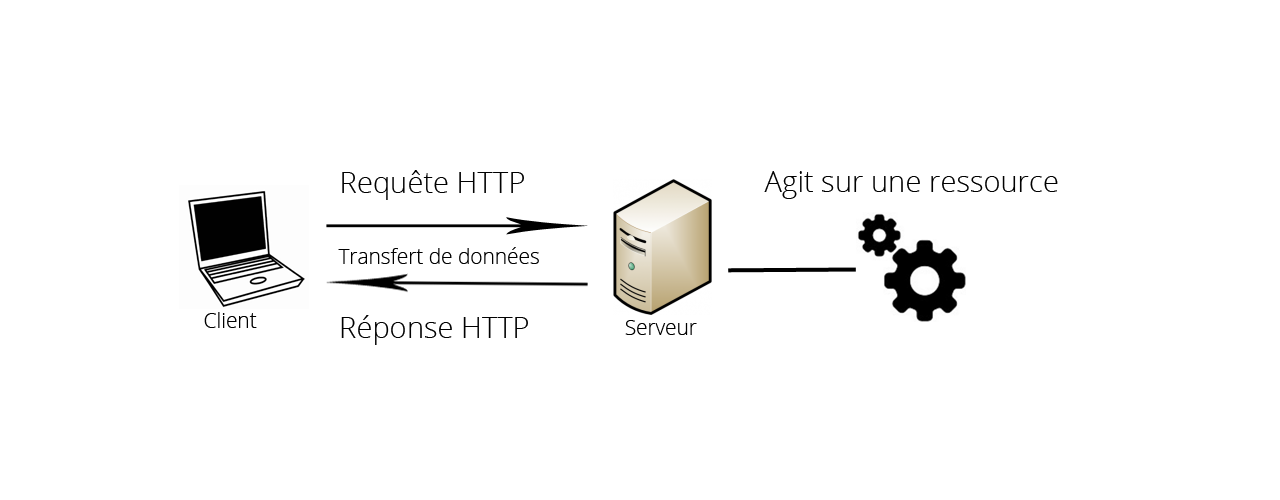
\includegraphics{http.png}}
\caption{Schéma de la communication avec HTTP entre un client et un serveur}\end{figure}

Nous devons utiliser ces requêtes lorsqu'il s'agit de modifier nos ressources, c'est-à-dire les enregistrements de notre base de données. Par exemple on crée un cours, on le modifie ou on le supprime. Le travail de RestLess est de supporter ces requêtes. En clair, il doit fournir une URL et une fonction qui s'occupent de traiter les différents types de requêtes. Attention à ne pas confondre, une requête n'agit pas directement sur une ressource, c'est le serveur qui s'en occupe. La requête consiste juste en un transfert de données entre le client et le serveur et ainsi elle déclenche des actions.


\subsection{Les classes RestLess}
\label{restless:les-classes-restless}
Maintenant que les bases sont en place, nous pouvons enfin nous intéresser à la liste des classes RestLess utilisées dans le projet avec les requêtes supportées et leur utilité.
\begin{itemize}
\item {} 
ListEndpoint
\begin{itemize}
\item {} 
get: retourne toutes les ressources

\item {} 
post: crée une nouvelle ressource

\end{itemize}

\item {} 
DetailEndpoint
\begin{itemize}
\item {} 
get: retourne une ressource

\item {} 
put: met à jour la ressource

\item {} 
delete: supprime la ressource

\end{itemize}

\item {} 
Endpoint
\begin{itemize}
\item {} 
pour créer des actions spécifiques

\end{itemize}

\end{itemize}

La liste ci-dessus regroupe les trois vues génériques dont nos classes peuvent hériter. Elles permettent de réaliser les quatre opérations sur nos ressources ainsi que des actions personnalisées. La différence entre la classe \code{DetailEndpoint} et \code{ListEndpoint} est que la première agit sur une ressource particulière. Elle a donc besoin d'un identifiant dans l'URL pour savoir quelle ressource elle doit modifier, dans le style \code{/courses/:id}. Notons qu'évidemment toutes les actions, le code qui s'exécute derrière une URL, retournent du JSON. En effet, il s'agit de la particularité et de l'utilité de RestLess. Comment concrètement utiliser ces classes dans le projet ? On fait comme précédemment dans l'exemple sur les vues génériques Django. La première étape consiste à créer une classe qui hérite soit de \code{ListEndpoint}, de \code{DetailEndpoint} ou de \code{Endpoint}. La seconde étape consiste à spécifier le modèle. Ensuite il faut créer une URL dans laquelle l'on spécifie qu'il faut utiliser notre classe précédemment déclarée. Ainsi. quand on fait une requête sur cette URL, suivant le type de requête, Django fait appel aux méthodes provenant des vues génériques RestLess. Par exemple, on crée une classe \code{CoursesList} dans laquelle on spécifie le modèle \code{Course}. Ensuite on rattache cette classe à l'url \code{/courses}. Si l'on fait une requête de type POST sur \code{/courses}, Django va chercher la méthode \code{post}, même nom que le type de requête, dans la classe \code{CoursesList}. Comme il ne la trouve pas dans notre classe, il la cherche dans la classe parente \code{ListEndpoint} et l'exécute. On appelle ce principe l'héritage. Le résultat est qu'une ressource est créée dans la table \code{courses} avec les paramètres du client. Une réponse en JSON contenant la ressource créée est retournée. On peut également faire une requête GET sur \code{/courses} et le serveur retourne tous les cours en format JSON également. Rien n'est plus nécessaire pour avoir notre API JSON fonctionnelle.
\begin{figure}[htbp]
\centering
\capstart

\scalebox{0.900000}{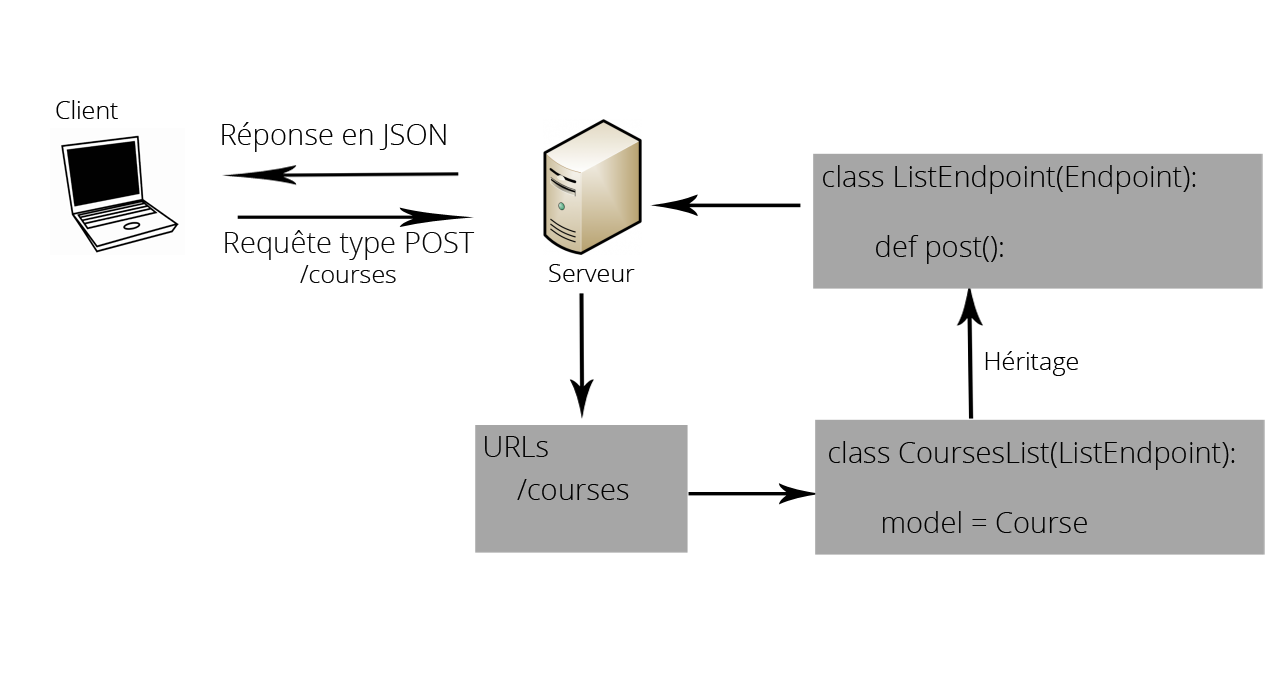
\includegraphics{requetes.png}}
\caption{Schéma du traitement d'une requête à l'aide des vues génériques RestLess}\end{figure}

Dans le cas de notre projet, il a fallu personnaliser les vues génériques pour répondre aux besoins spécifiques des ressources. Pour ce faire, il faut surcharger les méthodes héritées des classes RestLess. Comme mentionné précédemment, les méthodes ont le nom de la requête à laquelle elles correspondent. Si l'on fait une requête PUT, la méthode \code{put} est appelée et ainsi de suite. C'est un principe des vues génériques Django. En ce qui concerne les vues génériques, si notre classe ne contient pas le méthode appelée par une requête, le framework va automatiquement chercher la méthode dans la classe parente. Celle-ci est la classe RestLess qui contient les méthodes classiques et conventionnelles qui nous évitent un code redondant. En revanche, si l'on ne veut plus utiliser ces méthodes classiques car elles ne sont plus adaptées, l'on crée alors une méthode de même nom dans la classe fille. Cette méthode est desormais appelée à la place de celle de la classe mère. On appelle cela surcharger une méthode. Dans le projet, toutes les vues génériques sont écrites dans le fichier \code{api.py}. On peut y observer que plusieurs méthodes de tous types ont été surchargées. Il faut s'inspirer des méthodes RestLess que l'on surcharge pour que la nouvelle méthode accepte les bons arguments et retourne une réponse valide. On retrouve le fichier source sur \href{https://django-restless.readthedocs.org/en/latest/\_modules/restless/modelviews.html}{la documentation RestLess} \footnote{
\href{https://django-restless.readthedocs.org/en/latest/\_modules/restless/modelviews.html}{https://django-restless.readthedocs.org/en/latest/\_modules/restless/modelviews.html}. Consulté le 4 janvier 15.
}.
\begin{figure}[htbp]
\centering
\capstart

\scalebox{0.900000}{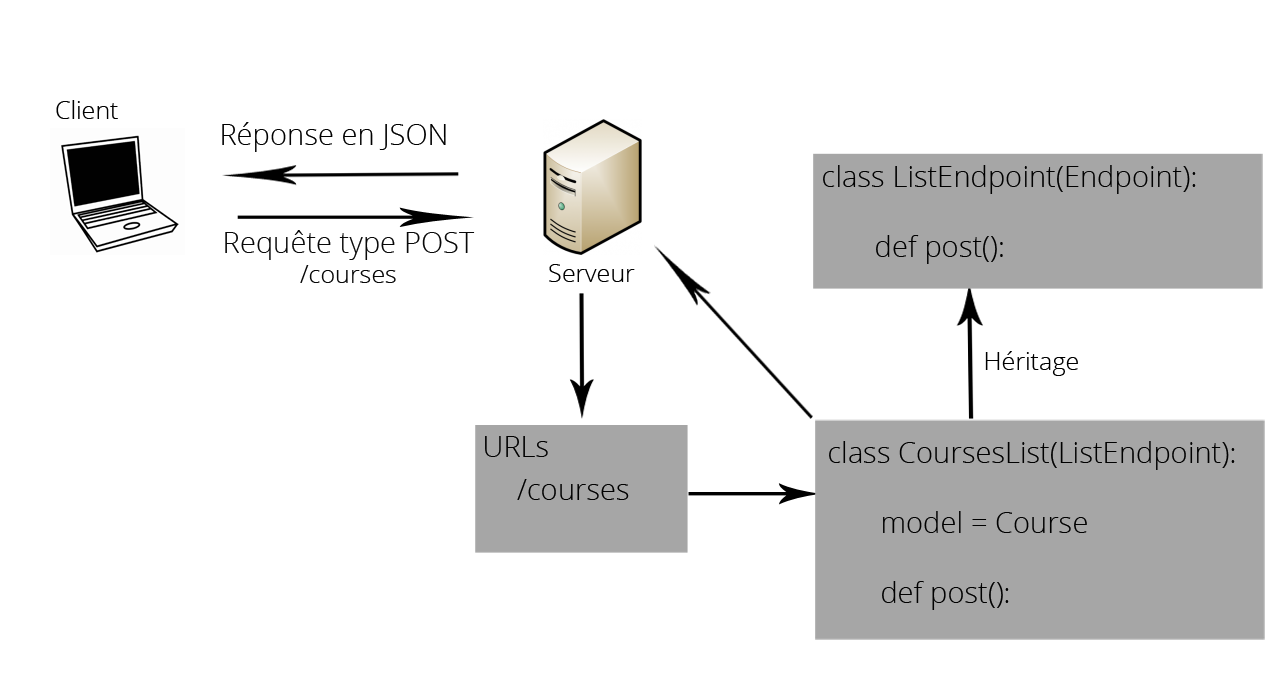
\includegraphics{surcharge.png}}
\caption{Surcharge d'une méthode}\end{figure}

On doit parfois retourner des objets JSON personnalisés, c'est-à-dire pouvoir choisir les paires clé/valeur de notre dictionnaire. Par défaut RestLess retourne simplement tous les attributs de l'enregistrement en question. On accomplit cette personnalisation généralement dans le but de choisir certains attributs, d'en créer des nouveaux qui ne sont pas des champs de la table ou de joindre des enregistrements associés. RestLess fournit la méthode \code{serialize} pour résoudre ce problème. Par exemple, pour un cours nous avons besoin de joindre les pages associées et leur contenu ainsi que le nombre total de pages. On peut se rendre sur \href{https://django-restless.readthedocs.org/en/latest/\#}{la documentation} \footnote{
\href{https://django-restless.readthedocs.org/en/latest}{https://django-restless.readthedocs.org/en/latest}. Consulté le 4 janvier 15.
} pour plus d'informations et sur le fichier \code{api.py} pour des exemples d'utilisation.


\subsection{Communication avec l'API}
\label{restless:communication-avec-l-api}
Nous avons construit une API JSON afin qu'AngularJS puisse communiquer avec une base de données. Pour effectuer les requêtes sur l'API, on trouve deux méthodes utilisées dans le projet. La première consiste à utiliser l'objet Angular \code{\$http}. Celui-ci permet de construire une requête et de récupérer la réponse ainsi que les éventuelles erreurs. On trouve toutes les spécifications sur la \href{https://docs.angularjs.org/api/ng/service/\$http}{documentation AngularJS} \footnote{
\href{https://docs.angularjs.org/api/ng/service/\$http}{https://docs.angularjs.org/api/ng/service/\$http}. Consulté le 21 mars 15.
}. La seconde méthode est d'utiliser l'objet \code{\$resource}. Si l'on possède une table sur laquelle on veut effectuer les opérations CRUD, \code{\$resource} nous évite d'écrire toutes les requêtes avec \code{\$http}. En effet, \code{\$resource} est un objet qui fournit directement les méthodes pour effectuer les différents types de requêtes sur l'API. Pour générer les URL, on fournit d'abord à l'objet une URL de base. Puis, en se basant sur les conventions du web, l'objet est capable d'effectuer les requêtes servant à agir sur la table. Ci-dessous se trouve un exemple d'un objet \code{\$resource} et de son utilisation partielle.

\begin{Verbatim}[commandchars=\\\{\}]
\PYG{k+kd}{var} \PYG{n+nx}{Section} \PYG{o}{=} \PYG{n+nx}{\PYGZdl{}resource}\PYG{p}{(}
    \PYG{l+s+s2}{\PYGZdq{}api/sections/:sectionId\PYGZdq{}}
\PYG{p}{)}\PYG{p}{;}

\PYG{n+nx}{Section}\PYG{p}{.}\PYG{n+nx}{query}\PYG{p}{(}\PYG{p}{)}\PYG{p}{;}
\PYG{c+c1}{// =\PYGZgt{} GET /api/sections}
\PYG{k+kd}{var} \PYG{n+nx}{section} \PYG{o}{=} \PYG{n+nx}{Section}\PYG{p}{.}\PYG{n+nx}{get}\PYG{p}{(}\PYG{p}{\PYGZob{}}\PYG{n+nx}{sectionId}\PYG{o}{:} \PYG{l+m+mi}{1}\PYG{p}{\PYGZcb{}}\PYG{p}{)}\PYG{p}{;}
\PYG{c+c1}{// =\PYGZgt{} GET /api/sections/1}
\PYG{n+nx}{card}\PYG{p}{.}\PYG{n+nx}{\PYGZdl{}save}\PYG{p}{;}
\PYG{c+c1}{// =\PYGZgt{} POST /api/sections/1}
\end{Verbatim}

Dans notre application, tous les objets \code{\$resource} sont définis dans le fichier \code{/courses/static/courses/javascripts/factories/resources.js}. La \href{https://docs.angularjs.org/api/ngResource/service/\$resource}{documentation} \footnotemark[5] fournit toutes les explications concernant \code{\$resource}.


\chapter{MathJax}
\label{maths:mathjax}\label{maths::doc}
\href{http://mathjax.org}{MathJax} \footnote{
\href{http://mathjax.org}{http://mathjax.org}. Consulté le 27 décembre 14.
} est un plugin JavaScript pour afficher des mathématiques dans le navigateur. Il utilise HTML et CSS pour afficher les expressions de mathématique dans le style LaTeX. Le rédacteur peut par conséquent aisément utiliser la notation LaTeX pour définir des fonctions, faire des fractions, des racines carrées, des puissances, écrire les symboles spéciaux, etc. en balisant le contenu et ensuite celui-ci sera correctement affiché grâce au moteur de rendu MathJax. Une section d'aide est disponible pour la syntaxe à utiliser.


\section{Installation}
\label{maths:installation}
L'installation de MathJax est très facile sur n'importe quelle site web. Il suffit de télécharger le dossier sur le \href{http://mathjax.org}{site officiel} \footnotemark[1], de le mettre dans le projet et d'inclure le lien du fichier JavaScript \code{MathJax.js} à la racine du dossier. Il est possible de charger une configuration différente de celle par défaut, pour changer la mise en forme, la notation et d'autres subtilités. On peut passer le nom de la configuration dans un paramètre \code{config} dans le lien qui inclut MathJax. Tous ces fichiers se trouvent dans le dossier \code{config} de MathJax. Il est aussi possible de créer sa configuration personnalisée. Les informations détaillées des configurations disponibles se trouvent dans \href{http://docs.mathjax.org/en/latest/config-files.html}{leur documentation} \footnote{
\href{http://docs.mathjax.org/en/latest/config-files.html}{http://docs.mathjax.org/en/latest/config-files.html}.  Consulté le 27 décembre 14.
}. Actuellement nous utilisons la configuration \code{TeX-AMS\_HTML} qui utilise la notation Tex (LaTeX) et qui génère du HTML. Il est aussi possible d'utiliser le CDN. On peut également spécifier dans le lien le fichier de configuration.

Une fois le plugin MathJax installé, il va automatiquement scanner les pages HTML et détecter les balises qui délimitent du contenu mathématique, par défaut \code{\$\$}. Ensuite il va mettre en forme le contenu afin qu'il s'affiche correctement. Ci-dessous se trouve un exemple de l'intégration du plugin et du résultat.

\begin{Verbatim}[commandchars=\\\{\}]
\PYG{n+nt}{\PYGZlt{}html}\PYG{n+nt}{\PYGZgt{}}
    \PYG{n+nt}{\PYGZlt{}head}\PYG{n+nt}{\PYGZgt{}}
        \PYG{c}{\PYGZlt{}!\PYGZhy{}\PYGZhy{}}\PYG{c}{ Fichiers locaux }\PYG{c}{\PYGZhy{}\PYGZhy{}\PYGZgt{}}
        \PYG{n+nt}{\PYGZlt{}script }\PYG{n+na}{src=}\PYG{l+s}{\PYGZdq{}/MathJax/MathJax.js?config=TeX\PYGZhy{}AMS\PYGZus{}HTML\PYGZdq{}}\PYG{n+nt}{\PYGZgt{}}\PYG{n+nt}{\PYGZlt{}/script\PYGZgt{}}

        \PYG{c}{\PYGZlt{}!\PYGZhy{}\PYGZhy{}}\PYG{c}{ CDN }\PYG{c}{\PYGZhy{}\PYGZhy{}\PYGZgt{}}
        \PYG{n+nt}{\PYGZlt{}script}
\PYG{n+nt}{            }\PYG{n+na}{src=}\PYG{l+s}{\PYGZdq{}http://cdn.mathjax.org/mathjax/latest/MathJax.js?config=TeX\PYGZhy{}AMS\PYGZus{}HTML\PYGZdq{}}\PYG{n+nt}{\PYGZgt{}}
        \PYG{n+nt}{\PYGZlt{}/script\PYGZgt{}}
    \PYG{n+nt}{\PYGZlt{}/head\PYGZgt{}}
    \PYG{n+nt}{\PYGZlt{}body}\PYG{n+nt}{\PYGZgt{}}
        \PYGZdl{}\PYGZdl{} f(x) = 5x + 4 \PYGZdl{}\PYGZdl{}
    \PYG{n+nt}{\PYGZlt{}/body\PYGZgt{}}
\PYG{n+nt}{\PYGZlt{}/html\PYGZgt{}}
\end{Verbatim}
\begin{figure}[htbp]
\centering
\capstart

\scalebox{0.500000}{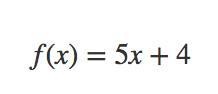
\includegraphics{mathjax.png}}
\caption{Résultat de MathJax}\end{figure}


\section{Personnalisation}
\label{maths:personnalisation}
Dans le cadre du projet, quelques modifications ont été faites par rapport à l'utilisation basique de MathJax. Pour pouvoir le personnaliser, on utilise un fichier spécial pour modifier les options que MathJax met à disposition. Ce fichier est déjà présent dans le dossier. Il se trouve dans le sous-dossier \code{config/local} et se nomme \code{local.js}. Ensuite, lorsque l'on inclut MathJax dans notre page, il suffit de modifier l'URL comme suit: \code{config=TeX-AMS\_HTML,local=local}. On a ajouté dans le paramètre \code{config} de l'URL \code{,local/local}.

Etudions ce fichier qui a été modifié pour les besoins du projet.

\begin{Verbatim}[commandchars=\\\{\}]
\PYG{n+nx}{MathJax}\PYG{p}{.}\PYG{n+nx}{Hub}\PYG{p}{.}\PYG{n+nx}{Config}\PYG{p}{(}\PYG{p}{\PYGZob{}}

    \PYG{n+nx}{skipStartupTypeset}\PYG{o}{:} \PYG{k+kc}{true}\PYG{p}{,}

    \PYG{c+c1}{// Apparence}
    \PYG{n+nx}{showProcessingMessages}\PYG{o}{:} \PYG{k+kc}{false}\PYG{p}{,}
    \PYG{n+nx}{messageStyle}\PYG{o}{:} \PYG{l+s+s2}{\PYGZdq{}none\PYGZdq{}}\PYG{p}{,}
    \PYG{n+nx}{showMathMenu}\PYG{o}{:} \PYG{k+kc}{false}\PYG{p}{,}
    \PYG{n+nx}{showMathMenuMSIE}\PYG{o}{:} \PYG{k+kc}{false}\PYG{p}{,}

    \PYG{n+nx}{styles}\PYG{o}{:} \PYG{p}{\PYGZob{}}
        \PYG{l+s+s2}{\PYGZdq{}.MathJax\PYGZus{}Display\PYGZdq{}}\PYG{o}{:} \PYG{p}{\PYGZob{}}
          \PYG{n+nx}{clear}\PYG{o}{:} \PYG{l+s+s2}{\PYGZdq{}both\PYGZdq{}}
        \PYG{p}{\PYGZcb{}}
    \PYG{p}{\PYGZcb{}}

\PYG{p}{\PYGZcb{}}\PYG{p}{)}\PYG{p}{;}

\PYG{n+nx}{MathJax}\PYG{p}{.}\PYG{n+nx}{Ajax}\PYG{p}{.}\PYG{n+nx}{loadComplete}\PYG{p}{(}\PYG{l+s+s2}{\PYGZdq{}[MathJax]/config/local/local.js\PYGZdq{}}\PYG{p}{)}\PYG{p}{;}
\end{Verbatim}

Premièrement, le groupe d'options commenté \code{Apparence} sert à supprimer les messages inutiles de MathJax, c'est-à-dire les messages de chargements par exemple. On supprime également le menu MathJax que celui-ci ajoute aux expressions qu'il transforme et que l'on affiche avec un clic droit. Ce menu est jugé inutile et surchargeant. Ensuite le dictionnaire \code{styles} permet d'ajouter du CSS en plus de celui que génère MathJax. On ajoute à la classe \code{MathJax\_Display}, une classe utilisée sur toutes les expressions qu'il transforme, le style \code{clear: "both"}. Il s'agit d'une correction d'un bug du plugin, car par défaut MathJax pouvait interférer avec le style déjà en place sur le site web. Ce problème créait des problèmes gênants pour l'interface. Finalement, la dernière configuration faite n'est pas la plus simple. Nous avons vu que MathJax analysait automatiquement toute la page HTML pour transformer le contenu balisé. Nous avons modifié ce comportement par défaut de MathJax. Il s'agit d'une part d'une question de performance. En effet, nous n'avons pas envie que des pages qui n'ont pas de contenu mathématique soient analysées par le lourd code JavaScript de MathJax. D'autre part, pour des questions de contrôle, l'on veut savoir exactement où il agit. L'option \code{skipStartupTypeset} permet donc de désactiver l'exécution automatique du processus MathJax. Le prochain défi est de trouver un moyen facilement utilisable pour indiquer quelle partie du code HTML doit être analysée. AngularJS a un outil très pratique pour accomplir ce genre de tâches. Nous avons déjà eu l'occasion de le découvrir dans le premier chapitre: {\hyperref[angularjs::doc]{\emph{les directives}}}. Ce sont des attributs ou éléments HTML qui exécutent des actions spécifiques, comme \code{ng-repeat} ou \code{ng-show}.

Nous allons donc créer une directive \code{mathjax}. Le code ci-dessous déclare simplement la directive.

\begin{Verbatim}[commandchars=\\\{\}]
\PYG{c+c1}{// on déclare la directive}
\PYG{n+nx}{app}\PYG{p}{.}\PYG{n+nx}{directive}\PYG{p}{(}\PYG{l+s+s1}{\PYGZsq{}mathjax\PYGZsq{}}\PYG{p}{,} \PYG{k+kd}{function}\PYG{p}{(}\PYG{p}{)} \PYG{p}{\PYGZob{}}
    \PYG{c+c1}{// Le code vient ici}
\PYG{p}{\PYGZcb{}}\PYG{p}{]}\PYG{p}{)}\PYG{p}{;}
\end{Verbatim}

Le but de cette directive est de pouvoir baliser les parties de notre page HTML qui contiennent des mathématiques. Par exemple, lorsque l'on affiche un cours, on aimerait faire de la façon suivante: \code{\textless{}mathjax\textgreater{}\{\{ cours.contenu \}\}\textless{}/mathjax\textgreater{}}.
Pour définir la directive et son comportement, il faut retourner un objet JavaScript contenant les options de notre directive. Ci-dessous se trouve la directive complète que nous allons analyser.

\begin{Verbatim}[commandchars=\\\{\},numbers=left,firstnumber=1,stepnumber=1]
\PYG{n+nx}{app}\PYG{p}{.}\PYG{n+nx}{directive}\PYG{p}{(}\PYG{l+s+s1}{\PYGZsq{}mathjax\PYGZsq{}}\PYG{p}{,} \PYG{k+kd}{function}\PYG{p}{(}\PYG{n+nx}{\PYGZdl{}timeout}\PYG{p}{)} \PYG{p}{\PYGZob{}}
    \PYG{n+nx}{restrict}\PYG{o}{:} \PYG{l+s+s1}{\PYGZsq{}AE\PYGZsq{}}\PYG{p}{,}
    \PYG{n+nx}{template}\PYG{o}{:} \PYG{l+s+s1}{\PYGZsq{}\PYGZlt{}div class=\PYGZdq{}ng\PYGZhy{}hide\PYGZdq{} ng\PYGZhy{}transclude\PYGZgt{}\PYGZlt{}/div\PYGZgt{}\PYGZsq{}}\PYG{p}{,}
    \PYG{n+nx}{transclude}\PYG{o}{:} \PYG{k+kc}{true}\PYG{p}{,}
    \PYG{n+nx}{link}\PYG{o}{:} \PYG{k+kd}{function}\PYG{p}{(}\PYG{n+nx}{scope}\PYG{p}{,} \PYG{n+nx}{element}\PYG{p}{,} \PYG{n+nx}{attrs}\PYG{p}{)} \PYG{p}{\PYGZob{}}
        \PYG{n+nx}{\PYGZdl{}timeout}\PYG{p}{(}\PYG{k+kd}{function} \PYG{p}{(}\PYG{p}{)} \PYG{p}{\PYGZob{}}
            \PYG{n+nx}{MathJax}\PYG{p}{.}\PYG{n+nx}{Hub}\PYG{p}{.}\PYG{n+nx}{Queue}\PYG{p}{(}\PYG{p}{[}\PYG{l+s+s2}{\PYGZdq{}Typeset\PYGZdq{}}\PYG{p}{,} \PYG{n+nx}{MathJax}\PYG{p}{.}\PYG{n+nx}{Hub}\PYG{p}{,} \PYG{n+nx}{element}\PYG{p}{[}\PYG{l+m+mi}{0}\PYG{p}{]}\PYG{p}{]}\PYG{p}{)}\PYG{p}{;}
            \PYG{n+nx}{MathJax}\PYG{p}{.}\PYG{n+nx}{Hub}\PYG{p}{.}\PYG{n+nx}{Queue}\PYG{p}{(}\PYG{k+kd}{function}\PYG{p}{(}\PYG{p}{)} \PYG{p}{\PYGZob{}}
                \PYG{n+nx}{element}\PYG{p}{.}\PYG{n+nx}{children}\PYG{p}{(}\PYG{p}{)}\PYG{p}{.}\PYG{n+nx}{removeClass}\PYG{p}{(}\PYG{l+s+s2}{\PYGZdq{}ng\PYGZhy{}hide\PYGZdq{}}\PYG{p}{)}\PYG{p}{;}
            \PYG{p}{\PYGZcb{}}\PYG{p}{)}\PYG{p}{;}
        \PYG{p}{\PYGZcb{}}\PYG{p}{)}\PYG{p}{;}
    \PYG{p}{\PYGZcb{}}
\PYG{p}{\PYGZcb{}}\PYG{p}{)}\PYG{p}{;}
\end{Verbatim}
\begin{itemize}
\item {} 
\textbf{restrict}: `AE' signifie que notre directive peut être un attribut (A = Attribut), avec le forme \code{\textless{}directive\textgreater{}\textless{}/directive\textgreater{}} ou un élément (E = Element), avec la forme \code{\textless{}div directive\textgreater{}\textless{}/div\textgreater{}}. On peut aussi ajouter l'option C pour utiliser la directive en tant que classe (C = Class), avec la forme \code{\textless{}div class="directive"\textgreater{}\textless{}/div\textgreater{}}.

\item {} 
\textbf{template}: Le contenu HTML dans notre directive.

\item {} 
\textbf{tranclude}: Cette option permet de récupérer le contenu qui est dans la directive et de le réinjecter dans le gabarit. En fait, par défaut, qu'importe le contenu de la directive sur la page HTML, celui-ci est de toute façon remplacé par la chaine de caractère de l'option \code{template}. Par exemple, si l'on écrit \code{\textless{}mathjax\textgreater{}\{\{ cours.contenu \}\}\textless{}/mathjax\textgreater{}}, le contenu du cours est supprimé. En revanche, quand on utilise l'option \code{transclude}, Angular récupère le contenu de la directive et l'injecte dans le gabarit de la directive, à l'endroit où l'on spécifie \code{ng-tranclude}. Ainsi on trouve dans l'option \code{template} le code HTML \code{\textless{}div ng-transclude\textgreater{}\textless{}/div\textgreater{}}. Le contenu de la directive est donc ajouté dans la \code{div}.

\item {} 
\textbf{link}: c'est la fonction qui est exécutée une fois que la page est compilée. En clair, quand AngularJS a transformé la page HTML et ses directives, le DOM est totalement généré. Ensuite seulement JavaScript peut agir sur celui-ci. Par conséquent, avec la fonction que l'on passe à \code{link}, on peut manipuler le contenu de notre directive. La fonction prend trois arguments. \code{scope} est basiquement l'objet qui contient les données du modèle. \code{element} est l'élément HTML lui-même et \code{attrs} contient les attributs HTML supplémentaires de notre directive.

\end{itemize}

Il y a encore beaucoup d'autres options disponibles pour personnaliser une directive, elles sont listées sur \href{https://docs.angularjs.org/guide/directive}{la documentation} \footnote{
\href{https://docs.angularjs.org/guide/directive}{https://docs.angularjs.org/guide/directive}. Consulté le 28 décembre 14.
}.

Intéressons nous maintenant au code qui se trouve à l'intérieur de la fonction \code{link}. La difficulté se trouve surtout dans le code spécifique à MathJax, \code{MathJax.Hub.Queue}. En fait, cette expression permet d'exécuter des fonctions en lien avec MathJax au bon moment. Elle permet tout simplement d'assurer que les fonctions que l'on passe à \code{Queue} s'exécutent une fois que MathJax est complétement chargé et qu'il est prêt à être utilisé. La première expression MathJax, à la ligne 7, indique qu'il faut analyser et mettre en forme le contenu de l'élément que l'on passe en argument, dans notre cas \code{element{[}0{]}}. On peut remarquer que l'on utilise \code{element{[}0{]}} et pas \code{element}. \code{element} est un objet contenant plusieurs informations tandis que \code{element{[}0{]}} retourne l'élément du DOM. Ensuite dans la deuxième expression, ligne 8, on enlève simplement la classe \code{ng-hide} de notre élément. Par défaut on cache le contenu de la directive, comme on peut l'observer dans l'option \code{template} qui contient la classe \code{ng-hide}. Cette expression sert à afficher la directive seulement une fois que les expressions mathématiques ont été transformées. Ainsi, l'utilisateur ne voit pas du contenu qui n'a pas encore été formaté par MathJax. Pour plus d'informations sur la \code{Queue} MathJax, on peut se rendre sur \href{http://docs.mathjax.org/en/latest/typeset.html}{la documentation officielle} \footnote{
\href{http://docs.mathjax.org/en/latest/typeset.html}{http://docs.mathjax.org/en/latest/typeset.html}.  Consulté le 28 décembre 14.
}. Finalement, le code est enveloppé dans une fonction \code{\$timeout} qui permet simplement d'assurer, lorsque notre directive est utilisée dans une boucle, que la boucle soit terminée avant que nous exécutions les transformations.

Notre directive est prête à être utilisée ! Maintenant, il suffit de l'utiliser pour mettre en forme notre contenu mathématique à l'endroit désiré.

\begin{Verbatim}[commandchars=\\\{\}]
\PYG{n+nt}{\PYGZlt{}body}\PYG{n+nt}{\PYGZgt{}}
    \PYG{n+nt}{\PYGZlt{}mathjax}\PYG{n+nt}{\PYGZgt{}}
        \PYGZdl{}\PYGZdl{} f(x) = 5x + 4 \PYGZdl{}\PYGZdl{}
    \PYG{n+nt}{\PYGZlt{}/mathjax\PYGZgt{}}
\PYG{n+nt}{\PYGZlt{}/body\PYGZgt{}}
\end{Verbatim}


\chapter{Tests}
\label{tests:tests}\label{tests::doc}
Une série de tests a été conçue afin de pouvoir garantir l'utilisation des fonctionnalités et faciliter les futurs apports au projet. Dans notre cas, il s'agit de tests système, \emph{end-to-end} en anglais. Ce type de tests signifie que l'on teste l'application dans son ensemble et d'un point de vue utilisateur. On ne va pas tester juste une partie du code comme dans des tests unitaires, mais l'on va simuler un utilisateur et naviguer sur notre site afin de s'assurer que les fonctionnalités sont opérationnelles.

AngularJS fournit un outil adapté pour tester ses applications qui se nomme \href{http://angular.github.io/protractor/\#/}{Protractor} \footnote{
\href{http://angular.github.io/protractor/\#/}{http://angular.github.io/protractor/\#/}. Consulté le 18 mars 15.
}. Ce programme nous permet d'écrire des tests adaptés à AngularJS. En fait, Protractor fournit des outils spécifiques au framework. Par exemple, il permet de sélectionner des éléments par leur modèle Angular, \code{ng-model="password"}. Protractor attend aussi automatiquement qu'Angular ait fini de préparer la page et que les requêtes AJAX soient terminées avant de faire les tests. Basiquement, un test consiste tout simplement à se rendre sur une page, à cliquer sur un bouton et à vérifier un résultat. On simule un utilisateur. Dans le projet, les tests se trouvent dans le dossier \code{courses/spec}. Le fichier \code{conf.js}  sert à configurer Protractor et les autres fichiers se terminant par \emph{\_spec.js} contiennent les tests. Chaque fichier correspond à une route de notre site. Prenons un exemple dans lequel l'on vérifie si l'utilisateur peut changer de page sur un cours.

\begin{Verbatim}[commandchars=\\\{\}]
\PYG{n+nx}{it}\PYG{p}{(}\PYG{l+s+s2}{\PYGZdq{}allows to switch pages\PYGZdq{}}\PYG{p}{,} \PYG{k+kd}{function}\PYG{p}{(}\PYG{p}{)} \PYG{p}{\PYGZob{}}
    \PYG{c+c1}{// On se rend sur la page}
    \PYG{n+nx}{browser}\PYG{p}{.}\PYG{n+nx}{get}\PYG{p}{(}\PYG{l+s+s2}{\PYGZdq{}http://localhost:3333/courses/\PYGZsh{}/1/view/1\PYGZdq{}}\PYG{p}{)}\PYG{p}{;}
    \PYG{c+c1}{// On clique sur le lien}
    \PYG{n+nx}{element}\PYG{p}{(}\PYG{n+nx}{by}\PYG{p}{.}\PYG{n+nx}{id}\PYG{p}{(}\PYG{l+s+s2}{\PYGZdq{}next\PYGZhy{}page\PYGZdq{}}\PYG{p}{)}\PYG{p}{)}\PYG{p}{.}\PYG{n+nx}{click}\PYG{p}{(}\PYG{p}{)}\PYG{p}{;}
    \PYG{c+c1}{// On s\PYGZsq{}attend à ce que le titre ait changé}
    \PYG{n+nx}{expect}\PYG{p}{(}\PYG{n+nx}{element}\PYG{p}{.}\PYG{n+nx}{all}\PYG{p}{(}\PYG{n+nx}{by}\PYG{p}{.}\PYG{n+nx}{binding}\PYG{p}{(}\PYG{l+s+s2}{\PYGZdq{}page.name\PYGZdq{}}\PYG{p}{)}\PYG{p}{)}\PYG{p}{.}\PYG{n+nx}{getText}\PYG{p}{(}\PYG{p}{)}\PYG{p}{)}\PYG{p}{.}\PYG{n+nx}{toEqual}\PYG{p}{(}\PYG{l+s+s2}{\PYGZdq{}Les équations\PYGZdq{}}\PYG{p}{)}\PYG{p}{;}
\PYG{p}{\PYGZcb{}}\PYG{p}{)}\PYG{p}{;}
\end{Verbatim}

Notre test commence par la fonction \code{it}, qui décrit ce que l'on teste, par exemple dans ce code l'on déclare que ``Cela permet de changer de pages''. Cette description est utile car elle nous permet de savoir rapidement ce qui est testé. Aussi, lorsqu'un test ne fonctionne pas, de savoir tout de suite quelle fonctionnalité ne marche plus. Ensuite dans la fonction \emph{it} on décrit une série d'étape. On se rend sur la page \code{courses/\#/1/view/1}, on trouve le lien avec l'id \code{next-page} et on clique dessus. A la fin du test, on écrit une ``attente'', c'est ce qui détermine si le test passe. Dans notre cas, l'on s'attend à ce que le nouveau titre de la page soit ``Les équations'', car on a changé de page en cliquant sur le bouton.

Pour lancer les tests écrits pour notre application, on lance la commande \code{python3 manage.py tests}. La commande se charge principalement de créer une base de données propre avec des données spécifiques et de lancer les serveurs. Une fois la commande lancée, une fenêtre de navigateur s'ouvrira et les tests défileront dedans comme si un utilisateur agissait. A la fin des tests, il suffit de revenir dans la console pour avoir le compte-rendu, les résultats.

La commande exécutera par défaut tous les tests se trouvant dans le dossier \code{courses/spec}. Pour changer ce comportement, on peut spécifier le fichier en argument: \code{python3 manage.py tests home\_spec.js}. Pour changer le dossier, par défaut \code{courses}, il faut le spécifier avec l'option \code{-{-}app}. Par exemple: \code{python3 manage.py tests -{-}app teachers}.


\chapter{Guide du développeur}
\label{guide::doc}\label{guide:guide-du-developpeur}

\section{Fichiers}
\label{guide:fichiers}
Cette section permet de s'y retrouver dans la multitude de fichiers du projet et de comprendre certains processus.
\begin{itemize}
\item {} \begin{description}
\item[{courses/}] \leavevmode\begin{itemize}
\item {} 
\textbf{admin.py}: permet de rajouter les modèles que l'on veut voir apparaitre et modifier dans la zone d'administration Django. \href{https://docs.djangoproject.com/fr/1.7/ref/contrib/admin/}{Documentation officielle} \footnote{
\href{https://docs.djangoproject.com/fr/1.7/ref/contrib/admin}{https://docs.djangoproject.com/fr/1.7/ref/contrib/admin}. Consulté le 14 mars 15.
}

\item {} 
\textbf{api.py}: regroupe toutes les vues génériques RestLess qui servent à construire l'API JSON nécessaire à l'application AngularJS. Les classes déclarées sont ensuite utilisées dans le fichier \code{urls.py}.

\item {} 
\textbf{forms.py}: déclare les formulaires Django nécessaires pour enregistrer les données d'une requête dans la base de données. Ils sont utilisés principalement dans le fichier \emph{api.py}. \href{https://docs.djangoproject.com/fr/1.7/topics/forms/}{Documentation officielle} \footnote{
\href{https://docs.djangoproject.com/fr/1.7/topics/forms/}{https://docs.djangoproject.com/fr/1.7/topics/forms/}. Consulté le 14 mars 15.
}

\item {} 
\textbf{models.py}: déclare les modèles de notre application. Contient également des méthodes d'instance pour certains modèles. \href{https://docs.djangoproject.com/fr/1.7/topics/db/models/}{Documentation officielle} \footnote{
\href{https://docs.djangoproject.com/fr/1.7/topics/db/models/}{https://docs.djangoproject.com/fr/1.7/topics/db/models/}. Consulté le 14 mars 15.
}

\item {} 
\textbf{urls.py}: contient les URL spécifiques à l'application. Elles sont ensuite ajoutées dans le fichier principal \code{webmath/urls.py}. La première url, de nom \code{index}, est le point de départ de notre application AngularJS. Le reste des routes est défini directement par AngularJS dans le fichier \code{courses/static/courses/javascripts/config/routes.js}. Dans \code{urls.py}, la deuxième url, de nom \code{pdf}, est celle qui génère le PDF d'un cours. Les routes qui suivent sont celles de l'API JSON qui utilisent les vues génériques du fichier \code{api.py}. \href{https://docs.djangoproject.com/fr/1.7/topics/http/urls/}{Documentation officielle} \footnote{
\href{https://docs.djangoproject.com/fr/1.7/topics/http/urls/}{https://docs.djangoproject.com/fr/1.7/topics/http/urls/}. Consulté le 14 mars 15.
}

\item {} 
\textbf{utils.py}: regroupe une série de fonctions utiles utilisées à travers l'application.

\item {} 
\textbf{views.py}: contient les vues Django. A l'instar des URL, il n'y a que deux fonctions, une qui est le point de départ de l'application et l'autre qui génère le PDF d'un cours. \href{https://docs.djangoproject.com/fr/1.7/topics/http/views/}{Documentation officielle} \footnote{
\href{https://docs.djangoproject.com/fr/1.7/topics/http/views/}{https://docs.djangoproject.com/fr/1.7/topics/http/views/}. Consulté le 14 mars 15.
}

\end{itemize}

\end{description}

\item {} 
\textbf{courses/templates/courses/}: contient le gabarit de base \code{courses.html} de notre application et le fichier Markdown \code{pdf.md} servant à générer le PDF d'un cours.

\item {} \begin{description}
\item[{courses/static/courses/}] \leavevmode\begin{itemize}
\item {} 
\textbf{html/}: contient tous les fichiers HTML utilisés par AngularJS. Les pages HTML sont reliées à une route dans le ficher \code{courses/static/courses/javascripts/config/routes.js} d'AngularJS qui s'occupe d'associer une route à un fichier HTML.

\item {} 
\textbf{images/}: contient les images utilisées pour le design de l'application.

\item {} 
\textbf{stylesheets/}: contient les feuilles de styles.

\end{itemize}

\end{description}

\item {} \begin{description}
\item[{courses/static/courses/javascripts/:}] \leavevmode\begin{itemize}
\item {} 
\textbf{config/routes.js}: déclare les routes principales de notre application avec AngularJS. \href{https://docs.angularjs.org/tutorial/step\_07}{Documentation officielle} \footnote{
\href{https://docs.angularjs.org/tutorial/step\_07}{https://docs.angularjs.org/tutorial/step\_07}. Consulté le 14 mars 15.
}

\item {} 
\textbf{controllers/}: déclare les contrôleurs AngularJS. Un fichier correspond à une route et son contrôleur. Ils sont utilisés dans le fichier \code{routes.js}.

\item {} 
\textbf{directives/}: déclare des directives AngularJS. \href{https://docs.angularjs.org/guide/directive}{Documentation officielle} \footnote{
\href{https://docs.angularjs.org/guide/directive}{https://docs.angularjs.org/guide/directive}. Consulté le 14 mars 15.
}

\item {} 
\textbf{factories/resources.js}: déclare des objets ressources qui permettent de communiquer facilement avec l'API. \href{https://docs.angularjs.org/api/ngResource/service/\$resource}{Documentation officielle} \footnote{
\href{https://docs.angularjs.org/api/ngResource/service/\$resource}{https://docs.angularjs.org/api/ngResource/service/\$resource}. Consulté le 14 mars 15.
}

\item {} 
\textbf{filters/}: déclare des filtres AngularJS. \href{https://docs.angularjs.org/guide/filter}{Documentation officielle} \footnote{
\href{https://docs.angularjs.org/guide/filter}{https://docs.angularjs.org/guide/filter}. Consulté le 14 mars 15.
}

\item {} 
\textbf{app.js}: point de départ, déclare l'application AngularJS principale ainsi que les modules avec leurs dépendances. C'est dans ces modules qu'on ajoute ensuite les filtres, contrôleurs, etc.

\item {} 
\textbf{extensions.js}: permet de personnaliser Showdown.js, la bibliothèque qui transforme le Markdown en HTML. \href{https://github.com/showdownjs/showdown}{Documentation officielle} \footnote{
\href{https://github.com/showdownjs/showdown}{https://github.com/showdownjs/showdown}. Consulté le 14 mars 15.
}

\end{itemize}

\end{description}

\item {} 
\textbf{spec/conf.js}: fichier de configuration de Protractor, le moteur de test.

\item {} 
\textbf{spec/}: contient les fichiers de tests end-to-end Protractor. Chaque fichier correspond à une route de l'application.

\item {} \begin{description}
\item[{management/commands/}] \leavevmode\begin{itemize}
\item {} 
\href{https://docs.djangoproject.com/fr/1.7/howto/custom-management-commands/}{Documentation officielle} \footnote{
\href{https://docs.djangoproject.com/fr/1.7/howto/custom-management-commands/}{https://docs.djangoproject.com/fr/1.7/howto/custom-management-commands/}. Consulté le 14 mars 15.
}

\item {} 
\textbf{seed.py}: commande qui crée des données de démonstration dans la base de données afin d'avoir une application fonctionnelle.

\item {} 
\textbf{tests.py}: commande qui lance les tests Protractor.

\end{itemize}

\end{description}

\item {} 
\textbf{webmath/test\_router.py}: Le routeur permet d'utiliser plusieurs bases de données avec Django. En l'occurrence, le routeur permet d'utiliser une base de données différente lorsqu'on lance les tests de notre application. \href{https://docs.djangoproject.com/fr/1.7/topics/db/multi-db/}{Documentation officielle} \footnote{
\href{https://docs.djangoproject.com/fr/1.7/topics/db/multi-db/}{https://docs.djangoproject.com/fr/1.7/topics/db/multi-db/}. Consulté le 15 mars 15.
}

\end{itemize}


\section{URL}
\label{guide:url}
Cette section regroupe une explication de toutes les URL de l'application. Toutes les URL se trouvent dans l'espace de nom \code{courses}, par exemple \code{/courses/help}. Lorsque un \code{\#} se trouve dans l'URL, cela signifie que c'est une URL définie par AngularJS.


\subsection{Utilisateurs}
\label{guide:utilisateurs}\begin{itemize}
\item {} 
\textbf{\#/}: Page d'accueil de l'application, on y trouve une liste des cours publiés. Ils peuvent être triés par catégories ou favoris.

\item {} 
\textbf{\#/new}: Page qui permet aux enseignants de créer un nouveau cours.

\item {} 
\textbf{\#/:course\_id/edit/:page}: Page d'édition d'un cours. L'enseignant peut y éditer le contenu de son cours, le publier ou le retirer.

\item {} 
\textbf{\#/:course\_id/preview/:page}: Prévisualise une page d'un cours. Lorsqu'un enseignant rédige un cours, il peut voir le résultat final grâce à cette page.

\item {} 
\textbf{\#/teacher/courses:} Liste de tous les cours du site, publiés ou non.

\item {} 
\textbf{\#/help}: Page qui fournit une aide aux rédacteurs concernant la syntaxe \emph{Markdown} et \emph{LaTex}.

\item {} 
\textbf{\#/:course\_id/edit}: Page qui permet de modifier les informations de base d'un cours, telles que le nom, la description ou la difficulté.

\item {} 
\textbf{\#/:course\_id/view/:page}: Page pour lire un cours. Le cours y est affiché, on peut naviguer à travers les pages, commenter le cours, etc.

\item {} 
\textbf{/pdf/:course\_id/*.pdf}: Renvoie un cours au format PDF pour pouvoir être téléchargé.

\item {} 
\textbf{\#/about}: Page d'information générale sur l'application.

\end{itemize}


\subsection{API}
\label{guide:api}
Les URLs de l'API sont dans l'espace de nom \code{api}, par exemple \code{/courses/api/themes}.
\begin{itemize}
\item {} 
\textbf{/courses/all}: renvoie une liste de tous les cours, publiés ou non.

\item {} 
\textbf{/courses}
\begin{itemize}
\item {} 
GET: renvoie tous les cours publiés.

\item {} 
POST: crée un nouveau cours.

\end{itemize}

\item {} 
\textbf{/courses/:id}
\begin{itemize}
\item {} 
PUT: met à jour un cours.

\end{itemize}

\item {} 
\textbf{/pages/:page\_id/courses/:course\_id}:
\begin{itemize}
\item {} 
GET: renvoie le contenu d'une page d'un cours.

\item {} 
PUT: met à jour le contenu d'une page.

\end{itemize}

\item {} 
\textbf{/themes}: renvoie une liste de tous les thèmes en incluant leurs chapitres respectifs.

\item {} 
\textbf{/pages/:page\_id/sections}
\begin{itemize}
\item {} 
POST: ajoute une section à une page d'un cours.

\end{itemize}

\item {} 
\textbf{/courses/:course\_id/pages}
\begin{itemize}
\item {} 
POST: ajoute une page à un cours.

\end{itemize}

\item {} 
\textbf{/sections/:id}
\begin{itemize}
\item {} 
DELETE: supprime une section.

\end{itemize}

\item {} 
\textbf{/courses/:course\_id/comments}
\begin{itemize}
\item {} 
GET: renvoie les commentaires d'un cours.

\item {} 
POST: ajoute un commentaire à un cours.

\end{itemize}

\item {} 
\textbf{/courses/:course\_id/menu}: Permet de construire le menu d'un cours en renvoyant le nom de ses pages et de leurs sections.

\item {} 
\textbf{/courses/:course\_id/publish}
\begin{itemize}
\item {} 
PUT: publie/retire un cours en changeant l'attribut \code{published} de \code{True} à \code{False} et vice-versa.

\end{itemize}

\item {} 
\textbf{/courses/:course\_id/favorite}
\begin{itemize}
\item {} 
PUT: ajoute/retire un cours au/des favoris de l'utilisateur.

\end{itemize}

\item {} 
\textbf{/pages/:page\_id/progression}
\begin{itemize}
\item {} 
POST: marque une page d'un cours comme comprise ou à relire pour l'utilisateur.

\end{itemize}

\end{itemize}


\section{Concepts}
\label{guide:concepts}

\subsection{Intégration d'AngularJS avec Django}
\label{guide:integration-d-angularjs-avec-django}
En dehors de l'API et des PDF, Django ne fournit qu'une seule route dans l'application. En effet, à partir de cette route, Angular s'occupe de gérer les autres routes et les gabarits. Concrètement, lorsque l'on charge une page de notre application, la requête va d'abord passer par la vue Django \code{index} déclarée dans le fichier \emph{views.py}. Cette vue s'occupe simplement d'afficher le gabarit \code{courses.html}. Ce fichier HTML est une maquette pour notre application, c'est-à-dire que son contenu est sur toutes les pages. Il contient le menu, l'inclusion des fichiers JavaScript et des feuilles de syle, ainsi que le pied de page. Dans la balise \code{body}, on a ajouté la directive Angular \code{ng-app=Courses}. On déclare qu'à l'intérieur de cette balise se trouve une application AngularJS nommée \code{CoursesApp}. Ainsi, une fois que Django a affiché le gabarit \code{courses.html}, Angular va insérer le contenu du bon fichier HTML dans la balise \code{body} selon l'URL et les routes écrites dans le fichier \code{routes.js}. La page finale est maintenant visible par l'utilisateur. Par exemple, si l'on se rend sur \code{courses/help}, Angular s'occupe de chercher le fichier \code{help.html} et d'insérer son contenu dans la balise \code{body} de \code{courses.html}. L'avantage de ce système est que lorsque l'on change de page, la vue Django n'est pas rappelée, mais seul le contenu de \emph{body} est mis à jour avec le contenu HTML approprié à l'URL. AngularJS rend ainsi notre site web plus rapide.


\chapter{Bogues et améliorations}
\label{bugs::doc}\label{bugs:bogues-et-ameliorations}

\section{Bogues}
\label{bugs:bogues}
Bogues éventuels dans l'application.
\begin{itemize}
\item {} 
L'intégration de la syntaxe Markdown n'a pas été totalement testée, il est possible que certaines formules ne marchent pas lors de l'affichage du cours.

\item {} 
La génération de PDF n'a également pas été complétement testée, il est également possible de trouver des bogues, comme avec les images ou  les mathématiques contenus dans les cours.

\end{itemize}


\section{Améliorations}
\label{bugs:ameliorations}\begin{itemize}
\item {} 
Implémentation complète de l'authentification

\item {} 
Possibilité de changer l'ordre des pages

\item {} 
Possibilité de téléverser des vidéos et des images

\item {} 
Proposer des exercices en lien avec le cours

\item {} 
Afficher des statistiques (progression, pages à relire, propositions...) dans le tableau de bord ``élève''

\item {} 
Possibilité pour les étudiants de demander des cours spécifiques

\item {} 
Possibilité de faire une recherche parmi les cours publiés

\end{itemize}


\chapter{Conclusion}
\label{conclusion::doc}\label{conclusion:conclusion}
Au terme du développement de l'application web, on remarque que l'on dispose d'un outil utilisable, car les fonctionnalités cruciales sont présentes. Finalement, il ne manque plus que l'apport des professeurs sur le site. En effet, même si le site fonctionne, il n'est rien sans le contenu ajouté par les rédacteurs. L'on est cependant forcé de reconnaitre qu'écrire un cours n'est pas évident et que la rédaction peut représenter un investissement de temps non négligable. La faiblesse se trouve donc dans le besoin incontestable de personnes qui s'impliquent.

Afin d'améliorer l'expérience des utilisateurs du site, il est encore possible d'implémenter quelques fonctionnalités. Actuellement, le problème le plus important réside dans l'authentification. Effectivement, pour l'instant, la mise en oeuvre de l'authentification est très limitées. Toutes les URL ne sont pas protégées, c'est-à-dire qu'un étudiant peut par exemple écrire et publier un cours. De plus, il faudrait masquer des boutons sur les pages selon l'utilisateur connecté, élève ou professeur par exemple. L'autentification n'a pas été complètement programmée à cause des difficultés supplémentaires qu'apporte AngularJS. Il y a un travail additionel à fournir, par rapport à une authentification faite exclusivement avec Django. Ensuite, l'on peut citer encore quelques fonctionnalités qui valent la peine d'être rajoutées. Notamment, la possibilité de téléverser et d'inclure des images ou des vidéos, directement depuis la page de rédaction. Cela apporterait un confort supplémentaires aux enseignants. En ce qui concerne les étudiants, il serait intéressant qu'ils puissent faire une recherche textuelle parmi tous les cours, ou alors qu'ils voient leurs statistiques et des suggestions dans leur tableau de bord.

L'on espère aussi qu'à l'avenir les différents sites web développés dans le cadre du travail de maturité puissent être mis ensemble, afin de former une plateforme d'e-learning cohérente et complète. Ainsi, cela pourrait être un réel atout pour l'enseignement.


\chapter{Bibliographie}
\label{bibliographie::doc}\label{bibliographie:bibliographie}

\section{Bibliographie}
\label{bibliographie:id1}
GREEN Brad \& SESHADRI Shyam, AngularJS, Sebastopol, O’Reilly Media, 2013, 183 p.

ALEXIS Pierre \& BERSINI Hugues, Apprendre la programmation web avec Python et Django, Paris, Eyrolles, 2012, 319 p.

LE GOFF Vincent, Apprenez à programmer en Python, Paris, OpenClassrooms, 2012, 382 p.


\section{Webographie}
\label{bibliographie:webographie}
Python: \href{https://docs.python.org/3/}{https://docs.python.org/3/}

Django: \href{https://www.djangoproject.com/}{https://www.djangoproject.com/}

AngularJS: \href{https://angularjs.org/}{https://angularjs.org/}

Protracor: \href{http://angular.github.io/protractor/\#/}{http://angular.github.io/protractor/\#/}

CSS \& HTML: \href{http://www.w3schools.com/}{http://www.w3schools.com/}

Bootstrap: \href{http://getbootstrap.com/}{http://getbootstrap.com/}

Restless: \href{https://django-restless.readthedocs.org/en/latest/}{https://django-restless.readthedocs.org/en/latest/}

Pandoc: \href{http://johnmacfarlane.net/pandoc/}{http://johnmacfarlane.net/pandoc/}

Showdown: \href{https://github.com/showdownjs/showdown}{https://github.com/showdownjs/showdown}

MathJax: \href{http://www.mathjax.org/}{http://www.mathjax.org/}

Git: \href{http://git-scm.com/}{http://git-scm.com/}


\chapter{Source des illustrations}
\label{illustration:source-des-illustrations}\label{illustration::doc}\begingroup
\let\clearpage\relax
\renewcommand*\listfigurename{Tables}
\listoffigures
\endgroup


\renewcommand{\indexname}{Index}
\printindex
\end{document}
